

\documentclass[10pt,a4paper]{report}
\usepackage[utf8]{inputenc}
\usepackage[english]{babel}
\usepackage{amsmath}
\usepackage{amsfonts}
\usepackage{amssymb}
\usepackage{graphicx}
\usepackage{enumerate}   
\usepackage{caption}
\usepackage{float}
\usepackage{dsfont}
\usepackage{csquotes}
\usepackage{tikz}
\usepackage{pgfplots}
\usepgfplotslibrary{groupplots}
\pgfplotsset{compat=1.16} 
\usepackage{array} 
\usepackage{booktabs}	% for horizontal lines
\usepackage{varwidth}% http://ctan.org/pkg/varwidth
\usepackage{csvsimple} % automatic table generation from csv files
\usepackage{comment}
\usepackage[style=draft]{biblatex}
\bibliography{../bibliography}

% Macros zum Setzen von Formeln
%-------------------------------

\newcommand{\gradient}[1]{\left(\nabla #1 \right)}
\newcommand{\hesse}[1]{\left(\nabla^2 #1 \right)}
 
% transponiert
\newcommand{\transpose}[1]{#1^\mathrm{T}}
% Exponentialfunktion
\newcommand{\e}{\mathrm{e}}
% Imagin�re Einheit
\newcommand{\I}{\mathrm{I}}
% Einheitsmatrix E
\newcommand{\II}{\vec{E}} 
% Ableitungen
\newcommand{\dd}{\mathop{}\!\mathrm{d}}
\newcommand{\Diff}[2]{\frac{\dd#1}{\dd#2}}
\newcommand{\DiffT}[1]{\Diff{}{t}#1}
\newcommand{\DDiff}[2]{\frac{\dd^2}{\dd#2^2}#1}
\newcommand{\DDiffT}[1]{\DDiff{#1}{t}}
\newcommand{\PartDiff}[2]{\frac{\partial #1}{\partial #2}}
\newcommand{\PartDiffT}[1]{\Diff{#1}{t}}
\newcommand{\PartDDiff}[2]{\frac{\partial^2 #1}{\partial #2^2}}
\newcommand{\PartDDiffT}[1]{\DDiff{#1}{t}}

\newcommand{\lie}[1]{\mathrm{L}_{#1}}
\newcommand{\ad}[1]{\mathrm{ad}_{#1}}

% Betrag und Norm
\newcommand{\abs}[1]{\mleft\vert#1\mright\vert}
\newcommand{\norm}[1]{\mleft\Vert#1\mright\Vert}

% Macro f�r die Abst�nde in Gleichungen mit Nebenbedingungen
\providecommand{\with}{\,, & \qquad}
% Satzzeichen nach Formeln
\providecommand{\FullStop}{\text{~\@.\xspace}}
\providecommand{\Comma}{\text{~,\xspace}}

% Klammern
\providecommand{\of}[1]{\mleft(#1\mright)}
\newcommand{\braces}[1]{\mleft(#1\mright)}
\newcommand{\set}[1]{\mleft\{#1\mright\}}

% Variante f�r \left. und \right\. ohne Abstand
\providecommand{\mleftdot}{\mleft.\kern-\nulldelimiterspace}
\providecommand{\mrightdot}{\mright.\kern-\nulldelimiterspace}

\let\originalleft\left
\let\originalright\right
\renewcommand{\left}{\mleft}
\renewcommand{\right}{\mright}



% Zahlenmengen
\newcommand{\numset}[1]{\mathbbm{#1}}

\newcommand{\eps}{\varepsilon}

% Operatoren
\DeclareMathOperator{\sign}{sgn}
\DeclareMathOperator{\rang}{rang}
\DeclareMathOperator{\Real}{Re}
\DeclareMathOperator{\Imag}{Im}
\DeclareMathOperator{\grad}{grad}
\DeclareMathOperator{\adj}{adj}
\DeclareMathOperator{\Span}{span}
\DeclareMathOperator{\asin}{asin}
\DeclareMathOperator{\acos}{acos}
\DeclareMathOperator{\atan}{atan}
\DeclareMathOperator{\asinh}{asinh}
\DeclareMathOperator{\acosh}{acosh}
\DeclareMathOperator{\atanh}{atanh}

\newcommand{\diag}{\operatorname*{diag}}
\renewcommand{\ker}{\operatorname*{Kern}}
\newcommand{\bild}{\operatorname*{Bild}}
\newcommand{\konst}{\operatorname*{konst.}}
\newcommand{\const}{\operatorname*{const.}}

% Makro f�r Vektoren (unterscheide griechische Buchstaben)
\DeclareRobustCommand{\vec}[1]{ 				
	\ifthenelse{\equal{#1}{\omega} \OR \equal{#1}{\varphi} \OR \equal{#1}{\alpha} \OR \equal{#1}{\beta} \OR \equal{#1}{\chi} \OR \equal{#1}{\delta} \OR \equal{#1}{\varepsilon} \OR \equal{#1}{\phi} \OR \equal{#1}{\epsilon} \OR \equal{#1}{\gamma} \OR \equal{#1}{\eta} \OR \equal{#1}{\iota} \OR \equal{#1}{\kappa} \OR \equal{#1}{\lambda} \OR \equal{#1}{\mu} \OR \equal{#1}{\nu} \OR \equal{#1}{\pi} \OR \equal{#1}{\theta} \OR \equal{#1}{\vartheta} \OR \equal{#1}{\rho} \OR \equal{#1}{\sigma} \OR \equal{#1}{\varsigma} \OR \equal{#1}{\tau} \OR \equal{#1}{\upsilon} \OR \equal{#1}{\xi} \OR \equal{#1}{\psi} \OR \equal{#1}{\zeta}}{
		% F�r griechische Kleinbuchstaben muss boldsymbol verwendet werden (deckt mathbf nicht ab)
		\boldsymbol{#1}
	}{
		% Alle anderen Symbole verwenden mathbf
		\mathbf{#1}
	}
}


%------------------------------
% Macros zur Verwendung im Text
%------------------------------

% Namen
%-------
\providecommand{\Maple}{\textsc{Maple}\xspace}
\providecommand{\Matlab}{\textsc{Matlab}\xspace}
\providecommand{\MatlabSimulink}{\textsc{Matlab/Simulink}\xspace}
\providecommand{\Doxygen}{\textsc{Doxygen}\xspace}

% +++ English
% .\@ is not treated as a full stop (important for the length of the whitespace
% afterwards. \@. is always treated as a full stop.)
\providecommand{\ie}{i.\,e.\@\xspace} 
\providecommand{\eg}{e.\,g.\@\xspace}
\providecommand{\cf}{cf.\@\xspace}

% +++ German
\providecommand{\zB}{z.\,B.\@\xspace}
\providecommand{\ZB}{Z.\,B.\@\xspace}
\providecommand{\bzw}{bzw.\@\xspace}
\providecommand{\bspw}{bspw.\@\xspace}
\AtEndOfClass{\renewcommand{\dh}{d.\,h.\@\xspace}}
\providecommand{\Dh}{D.\,h.\@\xspace}
\providecommand{\ua}{u.\,a.\@\xspace}
\providecommand{\sog}{sog.\@\xspace}
\providecommand{\usw}{usw.\@\xspace}
\providecommand{\etc}{etc.\@\xspace}
\providecommand{\ggf}{ggf.\@\xspace}
\providecommand{\ca}{ca.\@\xspace}
\providecommand{\uU}{u.\,U.\@\xspace}
\providecommand{\vgl}{vgl.\@\xspace}

% f�r W�rter mit Bindestrich. (Setzt einen Bindestrich, an dem nicht getrennt
% werden darf, l�sst aber die Trennung im folgenden Wort zu.)
\providecommand{\hypII}[2]{#1\nobreakdash-\hspace{0pt}#2}
\providecommand{\x}[1]{\hypII{$x$}{#1}}
\providecommand{\y}[1]{\hypII{$y$}{#1}}
\providecommand{\z}[1]{\hypII{$z$}{#1}}

%--- Zeilenhoehe in Tabellen -------------------------------------------------
% Mit dem Befehl \TabEqn kann eine Formel in einer Tabelle gesetzt werden
% (einfach nur die Formel in die Tabelle eingeben bringt die vertikale
% Ausrichtung irgendwie durcheinander)
% \ExtraTabEqnSpace ist der Platz, der oben und unter einer Formel eingef�gt
% wird
\AtEndOfClass{
\newcommand{\ExtraTabEqnSpace}{1ex}
\makeatletter
\newcommand*{\TabEqn}[1]{%
\begingroup
	\setbox\@tempboxa=\hbox{%
	#1%
	}%
	% Hinzufuegung von 1ex zu Hoehe (\ht)
	% und Tiefe (\dp) der Box.
	% Umweg ueber \dimen@ erforderlich,
	% da man \ht, und \dp nur etwas zuweisen,
	% aber nichts hinzufuegen kann.
	\setlength{\dimen@}{\ht\@tempboxa}%
	\addtolength{\dimen@}{\ExtraTabEqnSpace}%
	\setlength{\ht\@tempboxa}{\dimen@}%
	\setlength{\dimen@}{\dp\@tempboxa}%
	\addtolength{\dimen@}{\ExtraTabEqnSpace}%
	\setlength{\dp\@tempboxa}{\dimen@}%
	\usebox\@tempboxa
\endgroup
}
\makeatother
}

\newcommand\mycircle{\@currsize\tikz[baseline=(n.210),inner sep=0pt]%
  \node[line width=0.1em, circle,minimum size=0.7\baselineskip,draw](n){};%
  }
%\myfillcircle[zuf�llender Winkel in Grad]
\newcommand\myfillcircle[1][360]{%
  \@currsize\tikz[baseline=(n.210),inner sep=0pt]%
    \fill(0,0)%
      node[line width=0.1em, circle,minimum size=0.7\baselineskip,draw](n){}%
      --+(0,0.35\baselineskip)%
      arc[start angle=90,end angle=90+#1, radius=0.35\baselineskip];%
}


% new command for another subsection
\newcommand{\subsubsubsection}[1]{\paragraph{#1}\mbox{}\\}
\setcounter{secnumdepth}{4}
\setcounter{tocdepth}{4}

\title{Chapter 2 \& 3}
\author{Weber Jakob}

\begin{document}

\maketitle
\tableofcontents
%%%%%%%%%%%%%%%%%%%%%%%%%%%%%%%%%%%%%%%%%%%%%%%%%%%%%%%%%%%%%%%%%%%%%%%%%%%%%%%%%%%%%%%%%%%%%%%%%%%%%%%%%%%%%%%%%%
%%%%%%%%%%%%%%%%%%%%%%%%%%%%%%%%%%%%%%%%%%%%%%%%%%%%%%%%%%%%%%%%%%%%%%%%%%%%%%%%%%%%%%%%%%%%%%%%%%%%%%%%%%%%%%%%%%
\chapter{Fundamentals} \label{chap:fundamentals}

This chapter summarizes the fundamentals of regression. Excellent overviews can be found in the textbooks \cite{wood2017generalized}, \cite{fahrmeir2007regression}, \cite{friedman2001elements}. The shown fundamentals are strongly aligned with the presentation given in \cite{fahrmeir2007regression}. Section~\ref{sec:LinModel} gives an overview of the model assumptions used throughout this work, Furthermore, Section~\ref{sec:ModelSelection} outlines methods to evaluate and compare different models again each other in terms of complexity and accuracy. Section~\ref{sec:Splines} is devoted to the  spline definitions, Finally, in Section~\ref{sec:Splines} the so-called Structured Additive Regression is shown. It is basically the as

\section{Linear Models} \label{sec:LinModel}
%%%%%%%%%%%%%%%%%%%%%%%%%%%%%%%%%%%%%%%%%%%%%%%%%%%%%%%%%%%%%%%%%%%%%%%%%%%%%%%%%%%%%%%%%%%%%%%%%%%%%%%%%%%%%%%%%%

Given the data set $D = \{ (x^{(i)}_1, \dots, x^{(i)}_q; y^{(i)}), \ i = 1, \dots, n\}$ , we aim to model the relation between the inputs $x_1, \dots, x_q$ and the output $y$ with a function $f(x_1, \dots, x_q)$. Since this relationship is not exact, there will be a random part $\epsilon$. It is typically assumed that this part is additive and thus  
\begin{align} \label{eq:model-structure}
	y = f(x_{1}, \dots, x_{q}) + \epsilon.
\end{align}
%
We would like to estimate the unknown function $f$. For this, some assumptions on the model structure are made:

\begin{enumerate}
	\item \emph{The unknown function $f$ is a linear combination of the inputs}
	
	The function $f(x_1, \dots, x_q)$ is modeled as a linear combination of inputs, i.e. in the form 
	
	\begin{align} \label{eq:linCombOfInputs}
		f(x_1, \dots, x_q) = \beta_0 + \beta_1 x_1 + \dots + \beta_q x_q,
	\end{align}
	
	with unknown parameters $\beta_0, \dots, \beta_q$. Note that the model~(\ref{eq:model-structure}) is linear in its parameters as well as in its inputs. The parameter $\beta_0$ is called intercept or bias in the machine learning community, see \cite{bishop2006patternRecognition}. For centered data, i.e. the expected value $\text{E}(x^{(i)}) = 0$, the intercept is equal to zero and can be neglected. We introduce the input vectors $\transpose{\vec{x}} = [1, x_1, \dots, x_q] \in \mathbb{R}^{q+1}$ and the parameter vector $\transpose{\vec{\beta}} = [\beta_0, \beta_1, \dots, \beta_q] \in \mathbb{R}^{q+1}$ to obtain 
	\begin{align}
		y(x_1, \dots, x_q) = y(\transpose{\vec{x}}) = \transpose{\vec{x}} \vec{\beta}.
	\end{align}
		
	\item \emph{Additive errors}
	
	An additional assumption of linear models is additivity of errors, which means that	
	\begin{align} \label{eq:linModelOneDim}
		y = \transpose{\vec{x}} \vec{\beta} + \epsilon.
	\end{align}
	%
	This is reasonable for many practical applications, even though it appears quite restrictive. 
\end{enumerate}

To estimate the unknown parameters or coefficients $\vec{\beta}$, we define the output vector $\transpose{\vec{y}} = [y^{(1)}, \dots, y^{(n)}] \in \mathbb{R}^n$ and data error vector $\transpose{\vec{\epsilon}} = [\epsilon^{(i)}, \dots, \epsilon^{(n)}] \in \mathbb{R}^n$ as well as the design matrix  

\begin{align} \label{eq:design-matrix}
	\vec{X} = \begin{bmatrix}   1     & x^{(1)}_1 & \dots & x^{(1)}_q \\ 
								  	  \vdots &        &       & \vdots \\ 
				  		  		1     & x^{(n)}_1 & \dots & x^{(n)}_q  
		\end{bmatrix} \in \mathbb{R}^{n \times q+1}		
\end{align}

and generate $n$ equations like (\ref{eq:linModelOneDim}), which can be combined to 

\begin{align} \label{eq:LinearModel}
	\vec{y} = \vec{X}\vec{\beta} + \vec{\epsilon}.
\end{align}

We assume that the design matrix $\vec{X}$ has full column rank, i.e. $\mathrm{rank}(\vec{X}) = q + 1 = p$, implying linear independence of the columns of $\vec{X}$, which is necessary to obtain a unique estimator for the regression coefficients $\vec{\beta}$, see \cite{fahrmeir2007regression}.

Another necessary requirement is that the number of data points $n$ is larger or equal to the number of regression parameters $p$, which is equivalent to the statement that the linear system in (\ref{eq:LinearModel}) is not underdetermined.

In addition to the assumptions on the unknown function $f$, the necessary assumptions on the error term $\epsilon_i$ are the following \cite{fahrmeir2007regression}:

\begin{enumerate}
	\item \emph{Expectation of the error} \\
	The errors have a mean value of zero, i.e. $\text{E}(\epsilon^{(i)}) = 0$

	\item \emph{Variances and correlation structure of the errors} \\
	We assume constant error variance with $\text{Var} (\epsilon^{(i)}) = \sigma^2$. This property is called homoscedasticity. Additionally, we assume that the errors are uncorrelated, which means $\text{Cov} (\epsilon^{(i)}, \epsilon^{(j)}) = 0$ for $i \ne j$. The combination of these assumptions lead to the covariance matrix $\text{Cov}(\vec{\epsilon}) = \text{E} (\vec{\epsilon} \transpose{\vec{\epsilon}}) = \sigma^2 \vec{I}$.
	
	\item \emph{Assumptions on the input and design matrix}
	We have to distinguish two cases where the inputs are deterministic or stochastic, In most cases, the input and the output are stochastic and hence all model assumptions are conditioned on the design matrix~(\ref{eq:design-matrix}). That means that the input (x gehört noch transponiert, liefert aber fehler in latex) $\vec{x}^{(i)}T = [1, x_1^{(i)}, \dots, x_q^{(i)}]$ and the errors $\epsilon_i$ are not stochastically independent. For notational simplicity, we usually suppress the dependence on the design matrix.

	\item \emph{Gaussian errors} \\
	The errors follow at least approximately a normal distribution. Together with assumptions 1 and 2, we obtain that $\epsilon^{(i)} = \mathcal N(0, \sigma^2)$. 
\end{enumerate}

Summarizing, we have the following model assumptions:

\begin{equation}
	\text{E}(\vec{y}) = \vec{X} \vec{\beta} \\
\end{equation}
\begin{equation}
	\text{Cov} (\vec{y}) = \sigma^2 \vec{I}, \\
\end{equation}
%	
yielding 

\begin{equation} \label{eq:linModelAsDistribution}
	\vec{y} \sim \mathcal N(\vec{X} \vec{\beta}, \sigma^2 \vec{I}).
\end{equation}

A linear model with multiple input variables can therefore be interpreted as a multi-variate normal distribution with its mean vector given by $\vec{\mu} = \vec{X} \vec{\beta}$ and its covariance matrix given by $\sigma^2 \vec{I}$, i.e. to specify the linear model given in (\ref{eq:linModelAsDistribution}), we need to estimate the regression coefficients $\vec{\beta}$ and the variance $\sigma^2$.

%%%%%%%%%%%%%%%%%%%%%%%%%%%%%%%%%%%%%%%%%%%%%%%%%%%%%%%%%%%%%%%%%%%%%%%%%%%%%%%%%%%%%%%%%%%%%%%%%%%%%%%%%%%%%%%%%%
\subsection{Parameter Estimation}

The linear model given in (\ref{eq:linModelAsDistribution}) features the unknown parameters $\vec{\beta}$ and $\sigma$, which need to be estimated using the given data. In the following, the estimators $\hat{\vec{\beta}}$ and $\hat \sigma$ are introduced, and their statistical properties are derived. The two methods to estimate the regression parameters in the context of linear models are the method of Least Squares (LS) and the method of Maximum Likelihood (ML).  

\subsubsection{The Method of Least Squares} \label{subsubsec:Method-of-LS}

The unknown regression parameters $\vec{\beta} \in \mathbb{R}^p$ are estimated by minimizing the sum of squared error

\begin{align} \label{eq:MethodOfLS} 
	\text{LS}(\vec{y}, \vec{\beta}) &=  \lVert \vec{y} - \vec{X} \vec{\beta} \rVert^2_2 = \sum_{i=1}^n\epsilon_i^2 = \transpose{\vec{\epsilon}} \vec{\epsilon},
\end{align}
%
with respect to $\vec{\beta}$ \cite{friedman2001elements}. Rewriting~(\ref{eq:MethodOfLS}) leads to the least squares criterion

\begin{align} \label{eq:LS_derivation}
		\begin{split}
				\text{LS}(\vec{y}, \vec{\beta})  &=\transpose{(\vec{y} - \vec{X} \vec{\beta})}(\vec{y} - \vec{X} \vec{\beta}) \\ 
								 				&=\transpose{\vec{y}}\vec{y} - 2\transpose{\vec{y}}\vec{X} \vec{\beta} + \transpose{\vec{\beta}}    \transpose{\vec{X}} \vec{X} \vec{\beta}.
		\end{split}
\end{align}
%
The first-order necessary condition for optimality, cf. \cite{luenberger1984linear}, reads as

\begin{align} \label{eq:LS_1st_derivative}
	\frac{\partial \text{LS}(\vec{y}, \vec{\beta})}{\partial \vec{\beta}} = -2\transpose{\vec{X}} \vec{y} + 2\transpose{\vec{X}} \vec{X} \vec{\beta} = 0.
\end{align}
%
The second-order condition requires the Hessian to be positive-definite, i.e. 

\begin{align} \label{eq:LS_2nd_derivative}
	\frac{\partial^2 \text{LS}(\vec{y}, \vec{\beta})}{\partial \vec{\beta} \partial \transpose{\vec{\beta}}} = 2\transpose{\vec{X}}\vec{X} > 0.
\end{align}
%
Since the design matrix $\vec{X} \in \mathbb{R}^{n \times p}$ is assumed to have full rank, the matrix $ \transpose{\vec{X}}\vec{X}$ is positive definite. The least squares estimate $\hat{\vec{\beta}}_{LS}$ is hence obtained, see~(\ref{eq:LS_1st_derivative}), by solving the so-called \emph{normal equations}

\begin{align} \label{eq:NormalEquations}
	\transpose{\vec{X}} \vec{X} \vec{\beta} = \transpose{\vec{X}} \vec{y}.
\end{align}
%
Since $\transpose{\vec{X}}\vec{X}$ is positive definite, the \emph{normal equations} (\ref{eq:NormalEquations}) feature a unique solution given by the least squares estimator

\begin{align} \label{eq:LS_estimator}
	\hat{\vec{\beta}}_{LS} = (\transpose{\vec{X}}\vec{X})^{-1} \transpose{\vec{X}}\vec{y}.
\end{align}

\subsubsection{Maximum Likelihood Estimation}

Under the normality assumption, the likelihood is defined as \cite{wood2017generalized}

\begin{align} \label{eq:likelihood}
	\mathcal{L}(\vec{\beta}, \sigma^2) = \frac{1}{(2\pi\sigma^2)^{n/2}} \exp \Big( -\frac{1}{2\sigma^2}\transpose{(\vec{y} - \vec{X} \vec{\beta})}(\vec{y} - \vec{X} \vec{\beta}) \Big).
\end{align}
%
The log-likelihood is then given by

\begin{align} \label{eq:log_liklihood}
	l(\vec{\beta}, \sigma^2) = -\frac{n}{2}\log(2\pi) - \frac{n}{2}\log(\sigma^2) - \frac{1}{2\sigma^2}\transpose{(\vec{y} - \vec{X} \vec{\beta})}(\vec{y} - \vec{X} \vec{\beta}).
\end{align}
%
Thus, maximizing the log-likelihood $l(\vec{\beta}, \sigma^2)$ with respect to $\vec{\beta}$ is equivalent to minimizing the least squares criterion given in (\ref{eq:MethodOfLS}). The maximum likelihood estimator $\hat{\vec{\beta}}_{ML}$ is therefore equivalent to the least squares estimator $\hat{\vec{\beta}}_{LS}$ in (\ref{eq:LS_estimator}).

%%%%%%%%%%%%%%%%%%%%%%%%%%%%%%%%%%%%%%%%%%%%%%%%%%%%%%%%%%%%%%%%
\subsection{Estimation of the Variance $\sigma^2$}

The estimation of the variance $\sigma^2$ is necessary for the construction of confidence intervals of the regression parameters and for the construction of prediction intervals. It is further used in all kinds of statistical tests as well as in model selection approaches and model assessment criteria \cite{blobel2013statistische}.

\subsubsection{Maximum Likelihood Estimation}

The first-order necessary condition for optimality results in this case in 

\begin{align} \label{eq:log_likelihood_derivative_sigma}
	\frac{\partial l(\vec{\beta}, \sigma^2)}{\partial \sigma^2} = -\frac{n}{2\sigma^2} + \frac{1}{2\sigma^4}\transpose{(\vec{y} - \vec{X} \vec{\beta})}(\vec{y} - \vec{X}\vec{\beta}) = 0. 
\end{align}
%
Substituting the maximum likelihood estimator $\hat{\vec{\beta}}_{LS}$, given in~(\ref{eq:LS_estimator}), for $\vec{\beta}$ results in the maximum likelihood estimator 

\begin{align} \label{eq:sigma_ML}
	\hat \sigma^2_{ML} = 
		\frac{(\vec{y} - \vec{X} \transpose{\hat{\vec{\beta}}_{LS})}(\vec{y} - \vec{X} \hat{\vec{\beta}}_{LS})}{n} = \frac{\transpose{\hat{\vec{\epsilon}}} \hat{\vec{\epsilon}}}{n}.
\end{align}
%
This estimator for $\sigma^2$ is rarely used since it is biased, i.e. $\text{E}(\sigma^2_{ML}) \ne \sigma^2$, see \cite{fahrmeir2007regression}. 

\subsubsection{Restricted Maximum Likelihood Estimation}

The mean value of the sum of squared residuals is $\text{E}(\transpose{\hat{\vec{\epsilon}}} \hat{\vec{\epsilon}}) = (n - p)\sigma^2$. Hence, a less biased estimator $\hat \sigma^2$ for $\sigma^2$ is given by

\begin{align} \label{eq:sigma_REML}
	\hat \sigma^2_{REML} = \frac{1}{n-q} \transpose{\hat{\vec{\epsilon}}} \hat{\vec{\epsilon}}.
\end{align}
%
The restricted maximum likelihood estimator for the variance is in general less biased \cite{fahrmeir2007regression}. Therefore, it is the commonly used estimator for the variance $\sigma^2$.

%%%%%%%%%%%%%%%%%%%%%%%%%%%%%%%%%%%%%%%%%%%%%%%%%%%%%%%%%%%%%%%%%%%%%%%%%%%%%%%%%%%%%%%%%%%%%%%%%%%%%%%%%%%%%%%%%%
\subsection{The Hat Matrix}

Using the least squares estimator~(\ref{eq:LS_estimator}), we can estimate the mean of $\vec{y}$ by 

\begin{align} \label{eq:mean_of_y}
	\widehat{\text{E}(\vec{y})} = \vec{\hat{y}} = \vec{X} \hat{\vec{\beta}}_{LS}
\end{align}
%
Substituting~(\ref{eq:LS_estimator}) results in 

\begin{equation} \label{HatMatrix}
	\vec{\hat{y}} = \vec{X}(\transpose{\vec{X}} \vec{X})^{-1} \transpose{\vec{X}} \vec{y} = \vec{H} \vec{y},
\end{equation}
%
with the matrix $\vec{H} \in \mathbb{R}^{n \times n}$, which is called \emph{hat matrix}. Using the \emph{hat matrix}, we can express the residuals $\hat \epsilon^{(i)} = y^{(i)} - \hat y^{(i)}$ in matrix notation as

\begin{align} \label{eq:residal_with_hat_matrix}
	\hat{\vec{\epsilon}} = \vec{y} - \hat{\vec{y}} = (\vec{I} - \vec{H}) \vec{y}.
\end{align}
%
The \emph{hat matrix} $\vec{H}$ has the following useful properties:

\begin{itemize}
	\item $\vec{H}$ is symmetric.
	\item $\vec{H}$ is idempotent, i.e. $\vec{H}^2 = \vec{H}$.
	\item The rank of $\vec{H}$ is equal to its trace.
 	\item $\frac{1}{n} \le h_{ii} \le 1$, if all data points are different, i.e. $x^{(i)} \ne x^{(j)}$ for $i \ne j$. Here, $h_{ii}$ are the diagonal elements of $\vec{H}$.
	\item The matrix $(\vec{I} - \vec{H})$ is also idempotent and symmetric, with $\mathrm{rank}(\vec{I} - \vec{H}) = n - p$.
\end{itemize}

The hat matrix is used in model selection techniques like cross-validation as well as in outlier detection and in diagnostic plots for linear models.

%%%%%%%%%%%%%%%%%%%%%%%%%%%%%%%%%%%%%%%%%%%%%%%%%%%%%%%%%%%%%%%%%%%%%%%%%%%%%%%%%%%%%%%%%%%%%%%%%%%%%%%%%%%%%%%%%%
\section{Model Selection} \label{sec:ModelSelection}

Linear models are widely exploited for regression problems on large data sets $(n \gg 0)$, because the solution of the \emph{normal equations} (\ref{eq:NormalEquations}) can be computed efficiently even for large $n$. If these data sets also contain a large number of input variables $(q \gg 0)$, the situation becomes more complicated since possible interaction effects or correlation of input variables may occur. This interaction terms limits the, otherwise perfect, interpretability of the linear model. 

Therefore, we need techniques and criteria to select the \emph{best possible model} out of the variety of different models for a given data set. Model assessment criteria, see Section~\ref{subsec:MAC}, are used to compare different models while subset selection techniques, see Section~\ref{subsec:SSM}, give an algorithmic approach to model generation. Further, we can influence the estimated coefficients $\vec{\beta}$ directly via regularization, see Section~\ref{subsec:Regularization}. 

%%%%%%%%%%%%%%%%%%%%%%%%%%%%%%%%%%%%%%%%%%%%%%%%%%%%%%%%%%%%%%%%
\subsection{Model Assessment Criteria} \label{subsec:MAC}

One way of comparing various models, i.e models using different sets of inputs, is the use of model assessment criteria. Generally, model assessment criteria can be split in two components. The first one measures the goodness of fit, e.g. using the sum of squared errors, while the second measures the complexity of the model. Most model assessment criteria are based on the sum of expected squared prediction error (SPSE). Therefore, the derivation of the SPSE is given next. 

\subsubsection{Sum of Expected Squared Prediction Error}

given independent observations $y_i, \ i = 1, \dots, n$ and a subset of inputs $\{x_0=1, x_1, \dots, x_q\}$, we want to measure the prediction quality. The specific models are defined by numbers $M \subset \{0, 1, \dots, q\}$ of used inputs with corresponding design matrix $\vec{X}_M$. Moreover, $\vert M \vert$ is the caridnal number of M, i.e. the number of inputs included in the model. The least squares estimator for $\vec{\beta}$, cf. (\ref{eq:LS_estimator}), is then given by

\begin{align*}
	\hat{\vec{\beta}}_{M} = (\transpose{\vec{X}}_M \vec{X}_M)^{-1} \transpose{\vec{X}}_M \vec{y}.
\end{align*}
%
The data $\vec{y}$ can be interpreted as random variable. We can then define an estimator $\hat{\vec{y}}_M$ for the vector $\vec{\mu}$ of expectations $\mu^{(i)} = \text{E}(y^{(i)})$ by

\begin{align} \label{eq:SPSE-estimator-y}
	\vec{\hat{y}}_M = \vec{X}_M  \hat{\vec{\beta}}_M.
\end{align}
%
Moreover, it is easy to show that the following properties hold true:

\begin{enumerate}[(i)]
	\item $\text{E} (\vec{\hat{y}}_M) = \vec{X}_M (\transpose{\vec{X}}_M \vec{X}_M)^{-1}\transpose{\vec{X}}_M \text{E}(\vec{y})$
	\item $\text{Cov} (\vec{\hat{y}}_M) = \sigma^2 \vec{X}_M (\transpose{\vec{X}}_M \vec{X}_M)^{-1}\transpose{\vec{X}}_M$
	\item $\sum_{i=1}^n \text{Var}(\hat y^{(i)}_M) = \sigma^2 \text{tr}(\vec{X}_M (\transpose{\vec{X}}_M \vec{X}_M)^{-1} \transpose{\vec{X}}_M) = \sigma^2 \vert M \vert $
	\item Sum of Mean Squared Error
		\begin{equation}  
		\begin{split} 
		\text{SMSE} &= \sum_{i=1}^n \text{E}(\hat y^{(i)}_M - \mu^{(i)}_M)^2 \\
				    &= \sum_{i=1}^n \text{E}\Big( \big( \hat y^{(i)}_M - \text{E}(\hat y^{(i)}_M) \big) + \big(\text{E}(\hat y^{(i)}_M) - \mu^{(i)}_M \big) \Big)^2 \\
				    &= \vert M \vert\sigma^2 + \sum_{i=1}^n \big( \text{E}(\hat y^{(i)}_M) - \mu^{(i)}_M \big)^2.
		\end{split}
		\end{equation}
\end{enumerate}

Note that the estimator~(\ref{eq:SPSE-estimator-y}) can be regarded as a prediction of future observations

\begin{align}
	y^{(n+i)} = \mu^{(i)} + \epsilon^{(n+i)}
\end{align}
%
for new input data $\{x_1^{(i)}, \dots, x_q^{(i)}\}$. Thus, we can derive the SPSE as

\begin{equation}
\begin{split}
	\text{SPSE} &= \sum_{i=1}^{n} \text{E}(y^{(n+i)} - \hat y^{(i)}_M)^2 \\ 
				&= \sum_{i=1}^{n} \text{E}\big((y^{(n+i)} - \mu^{(i)}_M) - (\hat y^{(i)}_M - \mu^{(i)}_M)\big)^2 \\ 
				&= \sum_{i=1}^{n} \text{E}(y^{(n+i)} - \mu^{(i)}_M)^2 + 2\text{E} \big( (y^{(n+i)} - \mu^{(i)})(\hat y^{(i)}_M - \mu^{(i)}_M) \big) + \text{E}(\hat y^{(i)} - \mu^{(i)}_M)^2 \\
				&= \sum_{i=1}^{n}\text{E}(y^{(n+i)} - \mu^{(i)}_M)^2 + \sum_{i=1}^{n} \big(\text{E}(\hat y^{(i)}_M) - \mu^{(i)}_M \big)^2 \\ 
				&= n\sigma^2 + \text{SMSE} \\ 
				&= n\sigma^2 + \vert M \vert \sigma^2 + \sum_{i=1}^{n} \big(\text{E}(\hat y^{(i)}) - \mu^{(i)}_M \big)^2.
\end{split}
\end{equation}

The SPSE can be split into three parts:

\begin{enumerate}
	\item \emph{Irreducible Prediction Error Term}: $n\sigma^2$ \\
	This term cannot be reduced through model selection techniques since it only contains the number of data points $n$ and the variance $\sigma^2$.

	\item \emph{Variance Term}: $\vert M \vert \sigma^2$ \\
	The second term contains the number of used variables $\vert M \vert$ as well as the variance $\sigma^2$. It can therefore be reduced by using a smaller number of inputs.
	
	\item \emph{Squared Bias Term}: $\sum_{i=1}^{n} \big( \text{E}(\hat y^{(i)} - \mu^{(i)}_M) \big)^2$\\
	The last term can be interpreted as bias. It can be reduced by increasing the model complexity.
\end{enumerate}
%
The SPSE acts as an example of the bias-variance trade-off, which is characteristic for all statistical models. It states that by increasing the model complexity, the bias is reduced but instead the variance is increased. On the other hand, by decreasing model complexity, the variance of the model is reduced, but the bias is increased, see Figure~\ref{fig:bv-decomposition} \cite{bishop2006patternRecognition}.

\begin{figure}[H]
	\centering
	\begin{tikzpicture}
		\pgfplotstableread{../thesisplots/figs/bvd.txt}{\data}
		\begin{axis}[
			xlabel=Model Complexity,
			xmin=0, xmax=2.1, 
			x label style={at={(axis description cs:0.5,-0.05),anchor=south}},
			ylabel=Error,
			y label style={at={(axis description cs:-0.1,.5)},rotate=-90,anchor=south},
			ymin=0, ymax=40, 
			axis lines = left,
			ticks = none,
			legend entries={Bias Error, Variance Error, Total Error, Optimal Model},
			] 
			\addplot [red] table [x=x, y=bias] {\data};		  		
			\addplot [blue] table [x=x, y=variance] {\data};	
			\addplot [black] table [x=x, y=both] {\data};	  
			\draw (0.672, 8.9341) circle [gray, radius=2pt];
			\addplot[dashed, gray] coordinates{(0.672,0) (0.672, 8.9341)};
		\end{axis}	
	\end{tikzpicture}
	\caption{Bias-variance decomposition}
	\label{fig:bv-decomposition}
\end{figure}

%[https://en.wikipedia.org/wiki/Bias–variance_tradeoff](https://en.wikipedia.org/wiki/Bias%E2%80%93variance_tradeoff)

In practice, the true value for the SPSE is not accessible since $\mu^{(i)}$ and $\sigma^2$ are unknown. Therefore, we need to estimate the SPSE. This can be done by using one of the following two strategies:

\begin{enumerate}

	\item \emph{Estimate SPSE using new and independent data} \\	
	If new observations are available, the SPSE can be estimated by
	\begin{align}
		\widehat{\text{SPSE}} = \sum_{i=1}^n (y^{(n+i)} - \hat y^{(i)}_M)^2.
	\end{align}
	These new observations can also be some held-out validation data from a train-validation split of the given data. 
	
	\item \emph{Estimate SPSE using existing data} \\
	When using existing data, the estimate for the SPSE is given by the squared error and an additional  term depending on the estimated variance and the model complexity. The estimate is thus given by
	\begin{align}
		\widehat{\text{SPSE}} = \sum_{i=1}^n(y^{(i)} - \hat y^{(i)}_M)^2 + 2\vert M \vert \hat \sigma^2.
	\end{align}

\end{enumerate}

Typically, used model assessment criteria follow the basic idea of the SPSE, see \cite{fahrmeir2007regression}.

\subsubsection{Corrected Coefficient of Determination}

The corrected coefficient of determination $R^2_{corr}$ is an improvement over the coefficient of determination $R^2$, which is defined as 

\begin{align}
	R^2 = 1 - \frac{\sum_{i=1}^n ( y^{(i)} - \hat y^{(i)}_M )^2}{\sum_{i=1}^n (y^{(i)} - \bar y)^2},
\end{align}
%
where $\bar y$ is defined as the mean value of $\vec{y}$. The major drawback of $R^2$ is that it will never decrease when further inputs are included in the model, e.g. the $R^2$ of a model using $\{x_1, x_2, x_3\}$ is always larger or equal the $R^2$ of a model using $\{x_1, x_2\}$, even if the variable does not enhance the prediction quality. 

The corrected coefficient of determination $R_{corr}^2$ reduces this problem by an correction term depending on the  number of parameters and is given by
\begin{align}
	R_{corr}^2 = 1 - \frac{n-1}{n-p}(1-R^2).
\end{align}

The corrected coefficient of determination is a standard output parameter in many statistical programs and may be used to compare even models with different number of used variables \cite{fahrmeir2007regression}.

\subsubsection{Mallow's Cp}

Mallow's complexity parameter is based directly on the ideas specified for the estimation of the SPSE and is given by

\begin{align}
	\text C_p = \frac{\sum_{i=1}^n (y^{(i)} - \hat y^{(i)}_M)^2}{\hat \sigma^2} - n + 2 \vert M \vert.
\end{align}
%
A lower value of Mallow's $\text C_p$ corresponds to a better model fit \cite{fahrmeir2007regression}.

\subsubsection{Akaike Information Criterion}

The AIC is among the most used model assessment criteria and defined by

\begin{align}
	\text{AIC} = -2 l(\hat{\vec{\beta}}_{ML}, \hat \sigma^2_{ML}) + 2(\vert M \vert +1),
\end{align}
%
where $l(\hat{\vec{\beta}}_{ML}, \hat \sigma^2_{ML})$ is the value of the log-likelihood (\ref{eq:log_liklihood}) at its maximum, i.e. at $\hat{\vec{\beta}}_{ML}$ and $\hat{\sigma}_{ML}$. It is worth noting that the total number of parameters is $\vert M \vert + 1$ because the variance is also counted as parameter. The log-likelihood for a linear model assuming Gaussian errors is given by, cf. (\ref{eq:log_liklihood}),

\begin{align}
	-2l(\hat{\vec{\beta}}_{ML}, \hat \sigma_{ML}^2) = n \log(\hat \sigma_{ML}^2) + n.
\end{align}
%
Therefore, neglecting the constant $n$, the AIC evaluates to

\begin{align}
	\text{AIC} = n \log(\hat \sigma^2_{ML}) + 2(\vert M \vert + 1).
\end{align}
%
A lower value of the AIC means a to a better model fit \cite{fahrmeir2007regression}.

\subsubsection{Bayesian Information Criteria}

The BIC is similar to the AIC, but it penalizes more complex models much harder than the AIC. In its general form, it is given as 

\begin{align}
	\text{BIC} = -2l(\hat{\vec{\beta}}_{ML}, \hat \sigma^2_{ML}) + \log(n) (\vert M \vert + 1).
\end{align}
%
Again, assuming Gaussian errors for a linear model and neglecting the constant term $n$, the BIC evaluates to

\begin{align}
	\text{BIC} = n\log(\hat \sigma_{ML}^2) + \log(n)(\vert M\vert + 1).
\end{align}
%
A lower value of the BIC correspond to a better model fit \cite{fahrmeir2007regression}.

\subsubsection{Cross-validation} \label{subsubsec:Cross-validation}

The basic idea of cross-validations is to split the given data set into a training set to estimate the parameters and a validation set to assess the prediction quality. A special case of cross-validation is the "leave-one-out" cross-validation, where all but one data point are used for training and the model is then evaluated on this held-out data point. This seems to be quite expensive, since one needs to estimate one model per data point. However, in the context of linear models, it can be shown that the cross-validation score can be computed using one model trained on all data $\vec{y}$ and the \emph{hat matrix} $\vec{H}_M = \vec{X}_M (\transpose{\vec{X}}_M \vec{X}_M)^{-1} \transpose{\vec{X}}_M$. The cross-validation score is then given by

\begin{align} \label{eq:cross-validation}
	\text{CV} = \frac{1}{n} \sum_{i=1}^n \Big( \frac{y^{(i)} - \hat y^{(i)}_M}{1 - h_{ii,M}} \Big)^2.
\end{align}
%
where $h_{ii,M}$ denote the diagonal elements of the \emph{hat matrix} and $\hat y^{(i)}_M$ is defined as the prediction of the model for the input $\{x^{(i)}_1, \dots, x^{(i)}_q \}$. A lower cross-validation score corresponds to a better model fit \cite{golub1979}.

An approximation to the cross-validation score is given by the so-called generalized cross-validation score. It is mainly used in the context of non-parametric regression or when the hat matrix $\vec{H}_M$ is numerically expensive to compute. In the GCV score, the diagonal elements of the hat matrix $h_{ii,M}$ are replaced by the mean of the trace of $\vec{H}_M$. The GCV score is then given by

\begin{align} \label{eq:generalizied-cross-validation}
	\text{GCV} = \frac{1}{n}\sum_{i=1}^n \Big( \frac{y^{(i)} - \hat y^{(i)}_M}{1 - \text{trace}(\vec{H}_M)/n}\Big)^2.
\end{align}
%
The numerical advantage comes from the fact that the trace of a product of matrices is invariant to cyclical permutations, i.e.

\begin{align}
	\text{trace}(\vec{H}_M) = \text{trace}(\vec{X}_M(\transpose{\vec{X}}_M \vec{X}_M)^{-1} \transpose{\vec{X}}_M) =\text{trace}(\transpose{\vec{X}}_M \vec{X}_M (\transpose{\vec{X}}_M \vec{X}_M)^{-1}).
\end{align} 
%
The trace can therefore be computed from the product of two matrices of shape $p\times p$ \cite{fahrmeir2007regression}.

%%%%%%%%%%%%%%%%%%%%%%%%%%%%%%%%%%%%%%%%%%%%%%%%%%%%%%%%%%%%%%%%
\subsection{Subset Selection Methods} \label{subsec:SSM}

To make use of the various model assessment criteria, some algorithmic approach to model selection needs to be given. The most commonly used approaches are forward, backward and stepwise selction \cite{fahrmeir2007regression}. 

In forward selection, start with a candidate model, which includes a small number of variables. In each iteration of forward selection, an additional variable is added to the candidate model.  The added variable is the one with leads to the largest reduction of a predefined model assessment criteria. The algorithm stops, if no further reduction is achieved.

In backward selection, start with a candidate model, which includes all variables. In each iteration of backward selection, we eliminate the variable from the model which provides the largest reduction of a predefined model assessment criteria. The algorithm stops, if no further reduction is possible. 

In step-wise selection, forward and backward selection are combined to enable the inclusion and deletion of a variable in every operation. The algorithm stops, if no further reduction is possible.

%%%%%%%%%%%%%%%%%%%%%%%%%%%%%%%%%%%%%%%%%%%%%%%%%%%%%%%%%%%%%%%%
\subsection{Regularization} \label{subsec:Regularization}

Model selection can also be achieved using regularization techniques by directly influencing the parameters $\vec{\beta}$, which need to be estimated given a data set. In general, regularization restricts the parameter space by adding some penalty term depending on the complexity of the model to the least squares objective function according to (\ref{eq:MethodOfLS}). This leads to the penalized least squares (PLS) criterion

\begin{align} \label{eq:PLS_crit}
	\text{PLS}(\vec{y}, \vec{\beta}) = \lVert \vec{y} - \vec{X} \vec{\beta}\rVert^2_2 + \lambda \cdot \text{pen}(\vec{\beta}),
\end{align}
%
where $\lambda$ is the so-called smoothing parameter and $\text{pen}(\vec{\beta})$ is the penalty term describing the regularization technique. 

In Ridge regression, the penalty term in the penalized least squares criterion in (\ref{eq:PLS_crit}) is given by the squared weighted $L_2$-norm of the parameter vector $\vec{\beta}$, i.e. $\text{pen}(\vec{\beta}) = \lVert \vec{\beta} \rVert^2_{\vec{K}} = \transpose{\vec{\beta}} \vec{K} \vec{\beta}$ with penalty matrix $\vec{K} \in \mathbb{R}^{p \times p}$. The closed form solution reads as

\begin{align}
	\hat{\vec{\beta}}_{PLS} = \arg \min_{\vec{\beta}} \big(\text{PLS}(\vec{y}, \vec{\beta}) \big) = (\transpose{\vec{X}} \vec{X} + \lambda \vec{K})^{-1} \transpose{\vec{X}}\vec{y},
\end{align}
%
The additional penalty term in Ridge regression leads to smaller parameter estimates $\hat{\vec{\beta}}_{PLS}$ compared to the unpenalized estimate $\hat{\vec{\beta}}_{LS}$. For large values of the smoothing parameter $\lambda$, the parameter estimates will converge towards, but never reach, zero. 

Ridge regression is commonly used when the input dimension $q$ is high, i.e. the number of parameters $\beta_i$ is large, and also known as Tikhonov regularization \cite{hoerl1970ridge}. Note that it is also possible to use a nonlinear penalty matrix $\vec{K}(\vec{\beta})$ resulting in

\begin{align}
	\text{pen}(\vec{\beta}) = \lVert \vec{\beta} \rVert^2_{\vec{K}(\vec{\beta})} = \transpose{\vec{\beta}} \vec{K}(\vec{\beta}) \vec{\beta}.
\end{align}
%
However, the resulting penalized least squares problem  has no closed form solution and must be solved by an iterative approach. We start with an initial guess $\vec{\beta}^{[0]}$ and iterate for $k = 0, 1, 2, \dots$ the iteration

\begin{align} \label{eq:PLS-iterative-approach}
	\vec{\beta}^{[k+1]} = \big(\transpose{\vec{X}} \vec{X} + \lambda \vec{K}(\vec{\beta}^{[k]}) \big)^{-1} \transpose{\vec{X}} \vec{y}.
\end{align}
%
until $\vert \vec{\beta}^{[k+1]} - \vec{\beta}^{[k]} \vert \le \text{Tol}$ with $\text{Tol}$ being some given tolerance.

?? Convergence ??

%%%%%%%%%%%%%%%%%%%%%%%%%%%%%%%%%%%%%%%%%%%%%%%%%%%%%%%%%%%%%%%%%%%%%%%%%%%%%%%%%%%%%%%%%%%%%%%%%%%%%%%%%%%%%%%%%%
%%%%%%%%%%%%%%%%%%%%%%%%%%%%%%%%%%%%%%%%%%%%%%%%%%%%%%%%%%%%%%%%%%%%%%%%%%%%%%%%%%%%%%%%%%%%%%%%%%%%%%%%%%%%%%%%%%
\section{Splines} \label{sec:Splines}
	
A spline is a piecewise polynomial defined on a sequence of knots. This definition is quite general. Therefore, a large variety of splines exists, ranging from regression splines \cite{eubank1990regressionsplines}, over B-splines \cite{deBoor1978practicalGuideToSplines} to natural cubic splines and many more. We will focus on the definition of B-splines in Section~\ref{subsec:b-splines}, tensor-product B-splines as the multi-dimensional expansion of B-splines in Section~\ref{subsubsec:tp-splines}, and P-splines in Section~\ref{subsec:p-splines} \cite{deBoor1978practicalGuideToSplines} \cite{eilers1996flexible}.
%%%%%%%%%%%%%%%%%%%%%%%%%%%%%%%%%%%%%%%%%%%%%%%%%%%%%%%%%%%%%%%%%%%%%%%%%%%%%%%%%%%%%%%%%%%%%%%%%%%%%%%%%%%%%%%%%%
\subsection{B-Splines} \label{subsec:b-splines}

We put the focus on the definition and use of B-splines, which are constructed from polynomial pieces in a recursive manner. The B-spline $B_j^l(x)$ of degree $l$ is defined by means of the Cox-de Boor recursion formula as \cite{fahrmeir2007regression}

\begin{align} \label{eq:Bspline_recDef1}
	B_j^0(x) = \begin{cases} 1 & \text{for} \quad \kappa_j \le x < \kappa_{j+1} \\ 
					 		 0 & \text{otherwise} 
	\end{cases}
\end{align}
\begin{align} \label{eq:Bspline_recDef2}
	B_j^l(x) = \frac{x - \kappa_{j-l}}{\kappa_{j} - \kappa_{j-l}} B_{j-1}^{l-1}(x) + \frac{\kappa_{j+1} - x}{\kappa_{j+1} - \kappa_{j+1-l}} B_{j}^{l-1}(x)
\end{align}
%
given the knot sequence 

\begin{align}\label{eq:knot_sequence}
	K = \{\kappa_{1-l}, \kappa_{1-l+1}, \dots, \kappa_{m+l-1}, \kappa_{m+l}\}
\end{align}
%
with the $m$ interior knots $\kappa_1, \dots, \kappa_m$ and the $2l$ boundary knots \cite{fahrmeir2007regression}. 

An example of B-splines of order $l=0, 1, 2$ and $3$ is given in Figure~\ref{fig:spline-types-both}. The left chart shows the B-splines based on an equidistant sequence of knots. The B-spline $B^0$ is the zero function, except for $x \in [\kappa_1, \kappa_2]$ where it is equal to 1. The B-spline $B^1$ is the well known \emph{hat function}, being zero except for $x \in [\kappa_1, \kappa_3]$. It consists of two linear pieces, one defined from $\kappa_1$ to $\kappa_2$ and the other from $\kappa_2$ to $\kappa_3$. Everywhere else, $B^1$ is equal to zero. At the joining points, the values of the linear pieces are equal. The B-spline $B^2$ consists of three quadratic pieces, joining at the knots $\kappa_2$ and $\kappa_3$. At these point, the values of the quadratic pieces, as well as their first derivatives are equal. Finally, the B-spline $B^3$ consists of 4 cubic pieces with the joining points at $\kappa_2$, $\kappa_3$ and $\kappa_4$ at which respective cubic polynomials possess equal values as well as equal first and second derivatives. The right part of Figure~\ref{fig:spline-types-both} shows the same B-splines defined on a non-equidistant knot sequence. The basic properties of these B-splines are the same as for B-splines based on equidistant knots. 

\begin{figure}[h]
	\centering
	\begin{tikzpicture}
	\pgfplotstableread{../thesisplots/figs/spline-types-equidistant.txt}{\equidistant}
	\pgfplotstableread{../thesisplots/figs/spline-types-quantile.txt}{\quantile}
	\begin{groupplot}[
			group style = {group size = 2 by 1},
			width=0.5\columnwidth,
			]
			\nextgroupplot[
			xmin=0.05, xmax=0.55, 
			xticklabels={$\kappa_1$, $\kappa_2$, $\kappa_3$, $\kappa_4$, $\kappa_5$},			
			xtick={0.1, 0.2, 0.3, 0.4, 0.5},
			xtick align=outside,
			xtick pos = bottom,
			ytick pos = left,
			ytick align=outside,
			ymin=-0.05, ymax=1.05, 
			legend entries={{$B^0$}, {$B^1$}, {$B^2$}, {$B^3$}},
			] 
			\addplot [black, dashed] table [x=x, y= B0] {\equidistant};		  		
			\addplot [violet, densely dotted] table [x=x, y=B1]{\equidistant};	
			\addplot [blue, dotted] table [x=x, y=B2]{\equidistant};
			\addplot [red, densely dashed] table [x=x, y=B3]{\equidistant};	  			
			\nextgroupplot[
			xmin=0.05, xmax=0.55, 
			xticklabels={$\kappa_1$, $\kappa_2$, $\kappa_3$, $\kappa_4$, $\kappa_5$},			
			xtick={0.1, 0.2, 0.38, 0.46, 0.52 },
			xtick align=outside,
			xtick pos = bottom,
			ytick pos = left,
			ytick align=outside,
			ymin=-0.05, ymax=1.05, 
			legend entries={{$B^0$}, {$B^1$}, {$B^2$}, {$B^3$}},
			] 
			\addplot [black, dashed] table [x=x, y= B0] {\quantile};		  		
			\addplot [violet, densely dotted] table [x=x, y=B1]{\quantile};	
			\addplot [blue, dotted] table [x=x, y=B2]{\quantile};
			\addplot [red, densely dashed] table [x=x, y=B3]{\quantile};	  	
		\end{groupplot}
	\end{tikzpicture}
	\caption{B-splines of orders $l=0, 1, 2, 3$ for equidistant (left) and non-equidistant (right) knots}
	\label{fig:spline-types-both}
\end{figure}

The shown locality is a very attractive feature leading to an enhanced numerical stability compared to other types of splines. Some general properties of B-splines of degree $l$ are summarized in the following list:

\begin{itemize}
	\item It consists of $l+1$ polynomial pieces of degree $l$, e.g. a cubic spline ($l=3$) consists of 4 cubic pieces.
	\item The pieces join at $l$ inner knots.
	\item At these knots, the derivatives up to order $l-1$ are continuous.
	\item The B-spline is positive on the domain spanned by $l+2$ knots, everywhere else it is zero, e.g. for $l=2$, a sequence of 4 knots is necessary.
	\item At every given $x$, only $l+1$ B-splines are non-zero.
\end{itemize}

The collection of $d = m + l - 1$ B-splines of degree $l$ over a sequence $K$ of $m+2l$ knots is called B-spline basis. The $2l$-knots are the boundary knots while the $m$ knots are the interior knots. The knots can either be an equidistant sequence, which facilitates the construction and estimation of the coefficients, or a non-equidistant sequence \cite{eilers1996flexible}. For equidistant knots, we split the domain $[a,b]$ into $m-1$ intervals, i.e

\begin{align} \label{eq:equidistant-knots-interval}
	h = \frac{b - a} {m - 1}
\end{align}
%
and obtain the sequence

\begin{align} \label{eq:equidistant-knots-sequence}
	\kappa_j = a + h(j-1), \quad j=1, \dots, m.
\end{align} 
%
Non-equidistant knot placement can be obtained using quantile-based knots, i.e. by using the $(j-1)/(m-1)$-quantiles for $j=1, \dots, m$ of the observed inputs $x^{(1)}, \dots, x^{(n)}$ as knots. Using this approach, more knots are placed in the areas where lots of data is present \cite{fahrmeir2007regression}. The boundary knots are usually set to be apart from each other by at least the minimal knot distance. 


A function $f(x)$ can then be represented utilizing the basis function approach by 

\begin{align} \label{eq:bspline-bf-approach}
	f(x) = \sum_{j=1}^d B_j^l(x) \beta_j = \transpose{\vec{b}} \vec{\beta},
\end{align}
%
using the B-spline basis functions $B_j^l(x)$ of appropriate degree $l$ and the parameter vector $\transpose{\vec{\beta}} = [\beta_1, \dots, \beta_d] \in \mathbb{R}^{d}$. The basis functions can be given in vector notation as $\transpose{\vec{b}} = [B_1^l(x), \dots, B_d^l(x)]$. Using the set of data $D = \{ (x^{(i)}, y^{(i)}), \ i=1, \dots, n \}$, the B-spline basis for $d$ splines of degree $l$ is given by the matrix $\vec{B}$ as

\begin{align} \label{eq:bspline-basis-matrix}
	\vec{B} = \begin{bmatrix}
				B_1^l(x^{(1)}) & \dots & B_d^l(x^{(1)})  \\
				\vdots         &       & \vdots 		 \\
				B_1^l(x^{(n)}) & \dots & B_d^l(x^{(n)})  \\
	\end{bmatrix} \in \mathbb{R}^{n \times d}.
\end{align}
%
The $n$ equations~(\ref{eq:bspline-bf-approach}) can be arranged as a linear model in the form

\begin{align}
	\vec{y} = \vec{B} \vec{\beta}.
\end{align}
%
A further advantage of B-splines is that once the basis in (\ref{eq:bspline-basis-matrix}) is given, the parameter can be estimated using the Least Squares algorithm given in Section~\ref{subsubsec:Method-of-LS}. Therefore, the estimation is computationally efficient and easy to implement since closed-form solutions exists. Further, the advanced theoretical framework of linear models can be applied to use model selection and regularization approaches as well as to calculate e.g confidence intervals for the regression coefficients and the prediction.
B-splines of appropriate order $l > 2$ produce smooths curves, i.e. first and second order derivatives are continuous, where the smoothness is mostly determined by the number of splines used. Using a low number $d$, the curve will be quite smooth, but possess a large data error. When using a high number of splines $d$, the data error will be small but the variance of the curve will be large. This is an example of the bias-variance trade-off, a classical problem of regression and machine learning and further discussed in Section~\ref{subsec:1d-function-estimation}. It is therefore necessary to introduce some kind of regularization \cite{deBoor1978practicalGuideToSplines}.  

%%%%%%%%%%%%%%%%%%%%%%%%%%%%%%%%%%%%%%%%%%%%%%%%%%%%%%%%%%%%%%%%%%%%%%%%%%%%%%%%%%%%%%%%%%%%%%%%%%%%%%%%%%%%%%%%%%

\subsubsection{Tensor-Product Splines} \label{subsubsec:tp-splines}

Tensor-product splines can be seen as the multi-dimensional extension of uni-variate B-splines. We start with a B-spline basis, cf. (\ref{eq:bspline-basis-matrix}), for each dimension and construct the tensor-product spline from these. 

We examine an example for two input dimensions $x_1$ and $x_2$. Tensor-product splines can in general be constructed for arbitrary dimensions using the approach given below. Assume that we have B-spline bases available, i.e. $\vec{A} \in \mathbb{R}^{n \times d}$ and $\vec{B} \in \mathbb{R}^{n \times d}$ using the same number of splines $d$ for both bases and degree $l=3$, for representing the functions $f_1(x_1)$ and $f_2(x_2)$, cf. (\ref{eq:bspline-bf-approach}), given by

\begin{align}
	f_1(x_1) &= \sum_{i=1}^{d} A_i^l(x_1) \alpha_i  = \transpose{\vec{a}} \vec{\alpha}, \\
	f_2(x_2) &= \sum_{j=1}^{d} B_j^l(x_2) \beta_j = \transpose{\vec{b}} \vec{\beta}
\end{align}

where $\vec{\alpha} \in \mathbb{R}^{d}$ and $\vec{\beta} \in \mathbb{R}^{d}$ are the coefficient vectors and $A_i^l(x_1)$ and $B_j^l(x_2)$ are the basis functions for degree $l$ for the respective dimension. To allow the function $f_1(x_1)$ to smoothly vary with $x_2$, its coefficients $\alpha_i$ must vary smoothly with $x_2$. By using the already available basis for representing smooth functions in $x_2$, we can write

\begin{align}
	\alpha_i(x_2) = \sum_{j=1}^{d} B_j^l(x_2) \beta_{ij} 
\end{align}

which leads to

\begin{align} \label{eq:tps-basis-function-approach-detailed}
	f_{1,2}(x_1, x_2) = \sum_{i=1}^{d} \sum_{j=1}^{d} A_i^l(x_1) B_j^l(x_2) \beta_{ij}.
\end{align}

We can therefore combine the individual basis matrices to generated a new basis matrix for the tensor-product spline. For any set of data $\{x^{(i)}_{1}, x^{(i)}_{2} \}, \ i = 1, \dots, n$, the relationship between the basis matrix $\vec{X}$ of the tensor-product spline and the marginal basis matrices $\vec{A}$ and $\vec{B}$, cf. (\ref{eq:bspline-basis-matrix}), is given by 

\begin{align}
	\vec{X} = \vec{A} \otimes \vec{B}
\end{align}

where $\otimes$ indicates the use of the row-wise Kronecker product, $\vec{X} \in \mathbb{R}^{n \times d^2}$ denotes the tensor-product spline basis, $\vec{A} \in \mathbb{R}^{n \times d}$ denotes the B-spline basis for dimension $x_1$ and $\vec{B} \in \mathbb{R}^{n \times d}$ denotes the B-spline basis for dimension $x_2$. The basis matrix for the tensor-product spline is therefore given by the row-wise Kronecker product of the marginal basis matrices. \cite{wood2017generalized}  

We can then model a two dimensional function $f(x_1, x_2)$ using data $\{x_1^{(i)}, x_2^{(i)}; y^{(i)} \}, \ i=i, \dots, n$ as in (\ref{eq:bspline-bf-approach}) as

\begin{align} \label{eq:tpspline-bf-approach}
	f(\vec{x}_1, \vec{x}_2) = \vec{X} \vec{\gamma}
\end{align}

with the tensor-product spline basis matrix $\vec{X} \in \mathbb{R}^{n \times d^2}$ and the coefficient vector $\vec{\gamma} \in \mathbb{R}^{d^2}$. The coefficient vector is obtained by reordering $\beta_{ij}$ in (\ref{eq:tps-basis-function-approach-detailed}).

This approach can in theory be continued for as much input dimensions as required. In practice, modeling more than two input dimensions using tensor-product splines becomes infeasible because of the exponential increase of basis functions and therefore coefficients to estimate. 


\subsubsection{Additive Regression} \label{subsubsec:STAR}
%
%We have again some given data  and want to model the generally non-linear relationship between the input data $\{x^{(i)}_{1}, \dots, x^{(i)}_{q}\}$ and the output $y^{(i)}$ by some multi-dimensional function $f(x_1, \dots, x_q)$.  Using, e.g. high-dimensional tensor-product splines, to model the function is computationally expensive, since the number of regression coefficients increases exponentially.

To circumvent this problem, we now assume the restrictive structure of additive models, given by

\begin{align} \label{eq:addRegBaseEquation}
	f(x_1, \dots, x_q) = f_1(x_1) + \dots + f_q(x_q) + \epsilon.
\end{align}

for some given data $\{x^{(i)}_{1}, \dots, x^{(i)}_{q}; y^i\}, \ i = 1, \dots, n$.

Hence, we use one function $f_i(x_i)$ per input dimension. \cite{fahrmeir2007regression} Using the concepts introduced above, i.e. using B-splines to estimate the function $f_i(x_i)$, we obtain for each function a linear model

\begin{align} \label{eq:addRegBaseEquation-as-linModel}
	f_i(\vec{x}_i) = \vec{X}_{s_i} \vec{\beta}_{s_i}
\end{align}

where $\vec{X}_{s_i} \in \mathbb R^{n \times d_i}$ is the B-spline basis using $d_i$ splines for the smooth function $f_i(x_i)$ of input dimension $i$, $\vec{x}_i = \transpose{(x_i^{(1)}, \dots, x_i^{(n)})}$ is the data vector of input dimension $i$ and $\vec{\beta}_{s_i} \in \mathbb R^{d_i}$ are the coefficients to be estimated. 

The model given in (\ref{eq:addRegBaseEquation-as-linModel}) does not contain interaction terms between variables. Nevertheless, these can be easily introduced for 2 dimensions using tensor-product splines without an overflowing increase in the number of coefficients.

We can then write the additive model with interaction terms in matrix notation as 

\begin{align} \label{eq:STAR}
	\vec{y} = \vec{X}_{s_1} \vec{\beta}_{s_1} + \dots + \vec{X}_{s_q} \vec{\beta}_{s_q} + \sum_{j=1}^{q-1} \sum_{r>j}^{q} \vec{X}_{t_{j, r}} \vec{\beta}_{t_{j, r}} + \vec{\epsilon}
\end{align}

using the error term $\vec{\epsilon} \in \mathbb{R}^n$, the tensor-product spline bases $\vec{X}_{t_{j,r}} \in \mathbb{R}^{n \times d_j d_r}$ and the tensor-product spline basis coefficients $\vec{\beta}_{t_{j, r}}$. This can be solved using ordinary least squares. 

Using the notation in (\ref{eq:STAR}) the theoretical framework of linear models can be applied to the additive regression models, since (\ref{eq:STAR}) can be formulated as large linear model as

\begin{align} \label{eq:STAR-block-diag}
	\vec{y} = \vec{X} \vec{\beta} = 
	\begin{pmatrix}
		\vec{X}_{s_1} &   \vec{X}_{s_2} & \dots & \vec{X}_{s_q} & \vec{X}_{t_{1,2}} & \dots & \vec{X}_{t_{q-1, q}}    
	\end{pmatrix} \begin{pmatrix} \vec{\beta}_{s_1} \\ \vec{\beta}_{s_2} \\ \vdots \\ \vec{\beta}_{s_q} \\ \vec{\beta}_{t_{1,2}} \\ \vdots \\ \vec{\beta}_{t_{q-1, q}} \\
	\end{pmatrix}
\end{align}

with $\vec{X}$ as large design matrix and $\vec{\beta}$ as combined coefficient vector. Therefore, the assumptions given in Chapter \ref{sec:LinModel} on the error term, as well as on the model functions are used. \cite{fahrmeir2004penalized}

%%%%%%%%%%%%%%%%%%%%%%%%%%%%%%%%%%%%%%%%%%%%%%%%%%%%%%%%%%%%%%%%%%%%%%%%%%%%%%%%%%%%%%%%%%%%%%%%%%%%%%%%%%%%%%%%%%
\subsection{P-Splines} \label{subsec:p-splines}

P-splines use the concepts of regularization to produce smooth function estimations. In our context, a function is said to be smooth if its $2^{nd}$ derivative is continuous and does not vary much. They where introduced by Eilers and Marx in \cite{eilers1996flexible} to overcome the problem stated above. Eilers and Marx simplified and generalized the idea of Osullivan in \cite{osullivan1986penalties}, who introduced a smoothness penalty based on the integral of the squared second derivative of the estimated spline to penalized wiggly function estimates. They proposed to use equidistant knot placement and a penalty based on finite differences of order $D$ of the coefficients of adjacent B-splines as approximation of the derivative.

The difference operator  $\Delta^D$ of order $D$ for equidistant knot placement of B-splines is defined by

\begin{align} \label{eq:difference-operators}
	\begin{split}
		\Delta^1 \beta_j &= \beta_j - \beta_{j-1} \\
		\Delta^2 \beta_j &= \Delta^1(\Delta^1 \beta_j) = \beta_j - 2\beta_{j-1} + \beta_{j-2} \\ 
		\vdots \\ 
		\Delta^D \beta_j &= \Delta^1(...(\Delta^1 \beta_j))
	\end{split}
\end{align}

and in matrix notation for order $D=1$

\begin{align} \label{eq:d1-difference-matrix}
	\vec{D}_1 = 
	\begin{pmatrix} 
		-1& 1&       &        &   \\  
		&-1& 1     &        &   \\  
		&  &\ddots & \ddots &   \\ 
		&  &       & -1     & 1 
	\end{pmatrix} \in \mathbb R^{d-1\times d}
\end{align}

and order $D=2$

\begin{align} \label{eq:d2-difference-matrix}
	\vec{D}_2 = 
	\begin{pmatrix} 
		1& -2& 1& &    \\  
		& 1 & -2 & 1& \\ 
		&  & \ddots & \ddots  & \ddots \\ 
		& & & 1 & -2 & 1 
	\end{pmatrix} \in \mathbb R^{d-2\times d}.
\end{align}

For non-equidistant knot placement, the difference operator $\Delta^1$ is defined according to \cite{ferziger2008numerische} as

\begin{align} \label{eq:d1-operator-nonequidistant}
	\Delta^1 \beta_j = \frac{\beta_j - \beta_{j-1}}{\delta_{j, j-1}}
\end{align}

with the denominator given by 

\begin{align} \label{eq:delta-operator}
	\delta_{j, j-1} = \operatorname*{arg\, max}_x B_j^l(x) - \operatorname*{arg\, max}_x B_{j-1}^l(x)
\end{align}

for the B-spline basis functions $B_j^l(x)$ and $B_{j-1}^l(x)$ of degree $l$. 
The second order difference operator is further defined using the first order difference operator $\Delta^1$ as 

\begin{align} \label{eq:d2-operator-nonequidistant}
	\Delta^2 \beta_j = \frac{\Delta^1 \beta_{j+1} - \Delta^1 \beta_j}{\delta_{j+1,j}}.
\end{align}

In matrix form, the first order difference operator for non-equidistant knot placement is then given as

\begin{align} \label{eq:d1-matrix-nonequidistant}
	\vec{D_1} = \begin{pmatrix}
					\frac{-1}{\delta_{2,1}} & \frac{1}{\delta_{2,1}} &                         &  \\
										   & \frac{-1}{\delta_{3,2}} & \frac{1}{\delta_{3,2}} & \\
										   & 				        & 	\ddots                 & \ddots \\
										   &                        &                         & \frac{-1}{\delta_{k-1, k-2}} & \frac{1}{\delta_{k-1, k-2}} \\ 
	\end{pmatrix} \in \mathbb{R}^{d-1 \times d}
\end{align} 

and the second order difference operator for non-equidistant knot placement is given as

\begin{align} \label{eq:d2-matrix-nonequidistant}
	\vec{D}_2 = \begin{pmatrix}
\frac{1}{\delta_{3,2} \delta_{2,1}} & \frac{- \delta_{3,1}}{\delta_{3,2}^2 \delta_{2,1}} & \frac{1}{\delta_{3,2}^2}  &  \\
									& \frac{1}{\delta_{4,3} \delta_{3,2}} & \frac{- \delta_{4,2}}{\delta_{4,3}^2 \delta_{3,2}} & \frac{1}{\delta_{4,3}^2} \\
									&       & 	\ddots    & \ddots & \ddots \\
		&    &  & \frac{1}{\delta_{k-1, k-2} \delta_{k-2, k-3}} & \frac{-\delta_{k-1, k-3}}{\delta_{k-1, k-2}^2 \delta_{k-2, k-3}} & \frac{1}{\delta_{k-1, k-2}^2} \\ 
	\end{pmatrix} \in \mathbb{R}^{d-2 \times d}
\end{align}

using the definition of $\delta_{j, j-1}$ in (\ref{eq:delta-operator}). This leads to the penalized least squares formulation, similar to (\ref{eq:PLS_crit}),

\begin{align} \label{eq:OF_psplines}
	Q_{pslines}(\vec{y}, \vec{\beta}) = \lVert \vec{y} - \vec{X} \vec{\beta}\rVert^2 + \lambda_s \mathcal J_s(\vec{\beta};D)
\end{align}

where $\lVert \vec{y} - \vec{X} \vec{\beta} \rVert^2$ is the mean squared error on the data for the spline fit, $\mathcal J_s(\vec{\beta};D) = \transpose{\vec{\beta}} \transpose{\vec{D}}_D \vec{D}_D \vec{\beta}$ is the smoothness penalty term given by the matrix form of the knot placement dependent difference operator $\Delta^D$ of order $D$ and $\lambda_s$ is the smoothness parameter determining the effect of the smoothness penalty. The estimated coefficients $\hat{\vec{\beta}}$ are then given by the minimization of

\begin{align}
	\hat{\vec{\beta}} = \arg \min_{\vec{\beta}} Q_{psplines}(\vec{y}, \vec{\beta}).
\end{align}

The penalized least squares formulation in (\ref{eq:OF_psplines}) then yields

\begin{align}
	\hat{\vec{\beta}} = (\transpose{\vec{X}} \vec{X} + \lambda_s \transpose{\vec{D}}_D \vec{D}_D)^{-1} \transpose{\vec{X}} \vec{y}.
\end{align}

The main advantage of P-splines is their easy set up. This advantage is diminished if uneven knot placement is chosen, which is seen when comparing the matrix forms of the difference operators for the different knot placement types in e.g. (\ref{eq:d2-difference-matrix}) and (\ref{eq:d2-matrix-nonequidistant}). 

A smoothness penalty term for tensor-product splines can be constructed using the Kronecker product. For this, we need to define the term \emph{adjacent coefficients} for two dimensional tensor-product splines. As one dimensional splines cover the input space $\{x_1\}$, two dimensional tensor-product splines cover the input space $\{x_1, x_2\}$ via the knot placement. To facilitate the description, we restrict ourselves to equidistant knot placement. \cite{fahrmeir2007regression} An example for the definition of adjacent coefficients, also called neighborhood, is taken from \cite{fahrmeir2007regression} and given in Figure \ref{fig:tps-neighborhood}.

\begin{figure}[H]
	\centering
	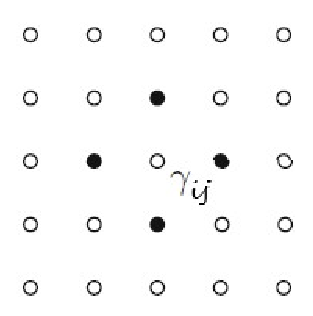
\includegraphics[width=0.2\columnwidth]{../thesisplots/tps-neighborhood-2cropped.pdf}
	\caption{Neighborhood or adjacent coefficients for tensor-product splines}
	\label{fig:tps-neighborhood}
\end{figure}

The adjacent coefficients to penalized for the coefficient $\gamma_{i,j}$, as in Chapter \ref{subsec:p-splines}, are therefore given by the coefficients left and right, i.e. $\gamma_{i-1,j}$ and $\gamma_{i+1, j}$, and the coefficients above and below, i.e. $\gamma_{i,j-1}$ and $\gamma_{i,j+1}$ for $i,j=1, \dots, d$. We now want to penalize adjacent coefficient differences in each dimension. We obtain the row-wise differences of order $D$ by applying the expanded difference matrix $\vec{I}^2 \otimes \vec{D}_D^1$ to the coefficient vector $\vec{\gamma}$, i.e.

\begin{align} \label{eq:tps-row-wise-differences}
	\transpose{\vec{\gamma}} \transpose{(\vec{I}^2 \otimes \vec{D}_D^1)} (\vec{I}^2 \otimes \vec{D}_D^1) \vec{\gamma} = \sum_{j=1}^d \sum_{i=1}^d (\gamma_{i,j} - \gamma_{i-1,j})^2 
\end{align}

using the identity matrix $\vec{I}^2 \in \mathbb{R}^{d \times d}$ of dimension $x_2$ and the difference matrix $\vec{D}_D^1$, cf. (\ref{eq:d1-difference-matrix}) and (\ref{eq:d2-difference-matrix}) for dimension $x_1$. The column wise differences are obtained analogously using the identity matrix $\vec{I}^1 \in \mathbb{R}^{d \times d}$ of dimension $x_1$ and the difference matrix $\vec{D}_D^2$. Summing up all column-wise and row-wise differences and using the properties of the Kronecker-product yields the penalty term $\mathcal{J}_s(\vec{\gamma}; D)$ as

\begin{align} \label{eq:tps-penalty-term}
	\mathcal{J}_s(\vec{\gamma}; D) = \transpose{\vec{\gamma}} \Big[ \vec{I}^2 \otimes \vec{K}_D^1 + \vec{K}_D^2 \otimes \vec{I}^1\Big] \vec{\gamma}
\end{align}

with the respective penalty matrices $\vec{K}_D^1 = \vec{D}_D^{1\text{T}} \vec{D}_D^1$ for dimension $x_1$ and $\vec{K}_D^2 = \vec{D}_D^{2\text{T}} \vec{D}_D^2$ for dimension $x_2$ of order $D$. 

With the penalty term in (\ref{eq:tps-penalty-term}), we can use the penalized least squares formulation, similar to (\ref{eq:PLS_crit}) and (\ref{eq:OF_psplines}). 

%%%%%%%%%%%%%%%%%%%%%%%%%%%%%%%%%%%%%%%%%%%%%%%%%%%%%%%%%%%%%%%%%%%%%%%%%%%%%%%%%%%%%%%%%%%%%%%%%%%%%%%%%%%%%%%%%%%%%%%%%%%%%%%%%%%%%%%%%%%%%%%%%%%%%%%%%%%%%%%%%%%%%%%%%%%%%%%%%%%%%%%%%%%%%%%%%%%%%%%%%%%%%%%%%%%%%%%%%%%%%%%%%%%%%%%%%%%%%%%%%%%%%%%%%%%%%%%%%%%%%%%%%%%%%%%%%%%%%%%%%%%%%%%%%%%%%%%%%%%%%%%%%%%%%%%%%%%%%%%%%%%%%%%%%%%%%%%%%%%%%%%%%%%%%%%%%%%%%%%%%%%%%%%%%%%%%%%%%%%%%%%%%%%

\chapter{Solution Approach} \label{chap:solution-approach}

We are now going to use the theory discussed in Chapter \ref{chap:fundamentals} to estimate functions using available data and a priori domain knowledge. An overview of the different problems considered in this work is given in Table \ref{tab:problem_overview}. First, we are using B-splines, see Chapter \ref{subsec:b-splines}, as basis functions for the estimation of the unknown function $y = f(x)$ for some data $\{x^{(i)}, y^{(i)}\} \ i = 1, \dots, n$.  Next, we use the concept of P-splines, see \ref{subsec:p-splines},  introduced by Eilers and Marx in \cite{eilers1996flexible} to estimate smooth, one dimensional functions. Finally, we are going to incorporate a priori knowledge into the fitting process using the approach given by Hofner and apply it to one and two dimensional functions. \cite{hofner2011monotonicity} 

\begin{table}[H]
	\centering
	\begin{tabular}{|lll|}
		\hline
		\textbf{Problem}                   & \textbf{Solution Approach}           & \textbf{Algorithm}  \\ \hline \toprule
		1d Function Estimation             & B-Splines                            & LS                  \\ \hline
		1d Smooth Function Estimation      & P-Splines                            & PLS                 \\ \hline
		1d Constraint Function Estimation  & P-Splines + Constraint Penalty       & PIRLS 			    \\ \hline 
		n-d Constraint Function Estimation & P+TP-Splines + Constraint Penalty & PIRLS 			    \\ \hline \bottomrule
	\end{tabular}
	\caption{Problem overview}
	\label{tab:problem_overview}
\end{table}

The a priori knowledge can be incorporated using different types of constraints. The considered constraints are listed in Table \ref{tab:constraint_overview}.

\begin{table}[h]
	\centering
	\begin{tabular}{|lll|}
		\hline
		\textbf{Constraint}& \textbf{Description}                         & \textbf{Math. Description}\\ \hline \toprule
		Monotonicity       & Functions is either increasing or decreasing.& $\lvert f'(x) \rvert \ge 0$ 	\\ \hline
		Curvature          & Function is either convex or concave.        & $\lvert f''(x) \rvert \ge 0$ 	\\ \hline
		Unimodality        & Function has a mode/peak.                    & $m = \arg \max_{x} f(x)$ 				\\ 
		&	   										  & $f'(x) \ge 0 \quad \text{if} \ x < m$  \\ 
		&  											  & $f'(x) \le 0 \quad \text{if} \ x > m$  \\ \hline
		Boundedness        & Function is bounded by the value M.          & $\lvert f(x)\rvert \le M$ 		\\ \hline
		Jamming            & Function is jammed by the value M.           & $f(x^{(M)}) \approx y^{(M)}$	\\ \hline \bottomrule
	\end{tabular}
	\caption{Overview of the considered constraints}
	\label{tab:constraint_overview}
\end{table}

To test the algorithm and the incorporation of a priori knowledge, we use the one dimensional function given by 

\begin{align}\label{eq:test_func}
	f(x) = 3\sin(3\pi x) + 17x + 3.
\end{align}

Figure \ref{fig:test_func} shows functions evaluated at 200 points. The function is partially increasing.  The test function for the two dimensional case is given in Chapter \ref{subsec:2d-example}. 

\begin{figure}[H]
	\centering
	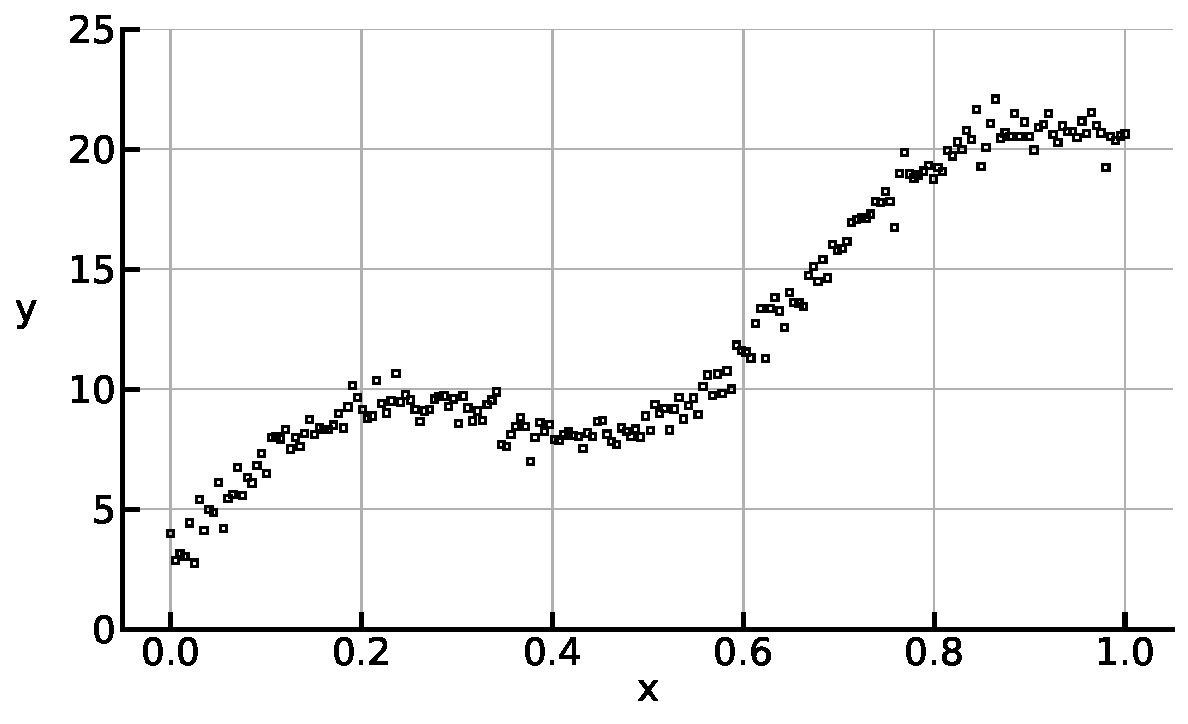
\includegraphics[width=\columnwidth]{../thesisplots/test_func.pdf}
	\caption{Noisy samples determined from test function (\ref{fig:test_func})}
	\label{fig:test_func}
\end{figure}

%%%%%%%%%%%%%%%%%%%%%%%%%%%%%%%%%%%%%%%%%%%%%%%%%%%%%%%%%%%%%%%%%%%%%%%%%%%%%%%%%%%%%%%%%%%%%%%%%%%%%%%%%%%%%%%%%
\section{Function Estimation}

\subsection{1d Function Estimation} \label{subsec:1d-function-estimation}

The goal is to model given data

\begin{align} \label{eq:data}
	\{\vec{x}, \vec{y}\} = \{x^{(i)}, y^{(i)}\}, \ i = 1, \dots, n 
\end{align}

using B-splines as basis functions. Therefore, we want to estimate the unknown function $\vec{y} = f(\vec{x})$, which can be represented as a linear combination of $k$ B-spline basis functions $B_j^m$ of degree $m=3$, cf. (\ref{eq:bspline-bf-approach}), as

\begin{align} \label{eq:basis_function_approach}
	\vec{y} = \vec{X} \vec{\beta},
\end{align}

where $\vec{X} \in \mathbb{R}^{n\times k}$ is the B-spline basis matrix, cf. (\ref{eq:bspline-basis-matrix}), and $\vec{\beta} \in \mathbb{R}^k$ are the coefficients to be estimated. 

The least squares objective function to be minimized using the complete data is then given by

\begin{align} \label{eq:OF_1}
	Q_1(\vec{y}, \vec{\beta}) = \lVert \vec{y} - f(\vec{x}) \rVert^2 = \lVert \vec{y} - \vec{X}\vec{\beta} \rVert^2 
\end{align}	

The coefficients are determined ive function $Q_1$ given in (\ref{eq:OF_1}) with respect to $\vec{\beta}$, i.e.

\begin{align}\label{eq:optimization_problem_1}
	\hat{\vec{\beta}}_{LS} = \arg \min_{\vec{\beta}} Q_1(\vec{y}, \vec{\beta}).
\end{align}

Using the least squares algorithm LS, see Chapter \ref{subsubsec:Method-of-LS}, the minimization problem (\ref{eq:optimization_problem_1}) yields 

\begin{align} \label{eq:LS_coef}
	\hat{\vec{\beta}}_{LS}= (\transpose{\vec{X}} \vec{X})^{-1} \transpose{\vec{X}} \vec{y}.
\end{align} 


Figure \ref{fig:smooth_bf} shows a B-spline model using $k=10$ splines on an equidistant grid approximating the noisy data presented in Figure \ref{fig:test_func}, as well as the individual cubic ($m=3$) B-spline basis functions $B_i^3(\vec{x})$ multiplied with the corresponding, estimated coefficients $\hat{\vec{\beta}}_{LS, j} \ j=1, \dots, 10$.

\begin{figure}[H]
	\centering
	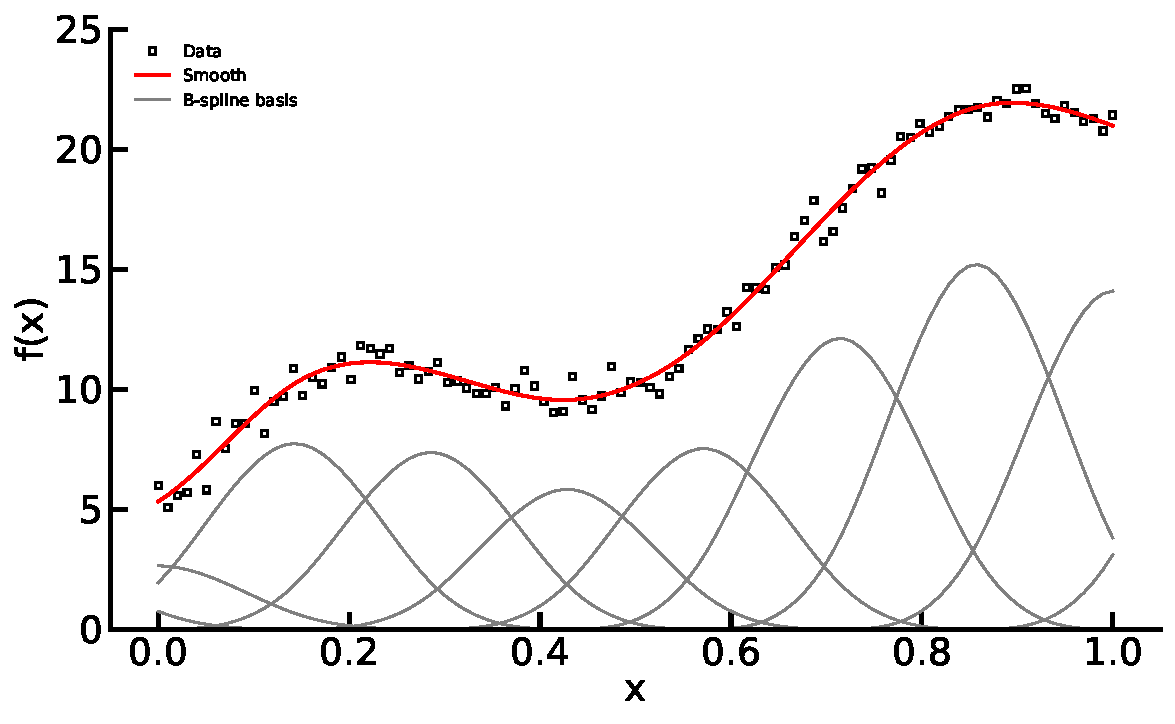
\includegraphics[width=\columnwidth]{../thesisplots/smooth_bf.pdf}
	\caption{Approximation of the noisy data by B-splines without constraints}
	\label{fig:smooth_bf}
\end{figure}


Note, the number of splines $k$ has a strong influence on the amount of smoothing. A small number $k$ leads to a very smooth estimate, but a large data error. On the other hand, when the number of splines is relatively large, the data error is very small but the smoothness of the estimate is poor. This behavior is an example of the well-known bias-variance dilemma and depicted in Figure \ref{fig:smooth_bf_large}. \cite{sammut2011}
Here, two B-splines models with $k=10$ and $k=50$ are illustrated, which are applied to the noisy data shown in Figure \ref{fig:test_func}. To overcome this challenges, the B-splines will be extended by penalizing the second derivative of the estimation, see Chapter \ref{subsec:1D_smooth}. 

\begin{figure}[H]
	\centering
	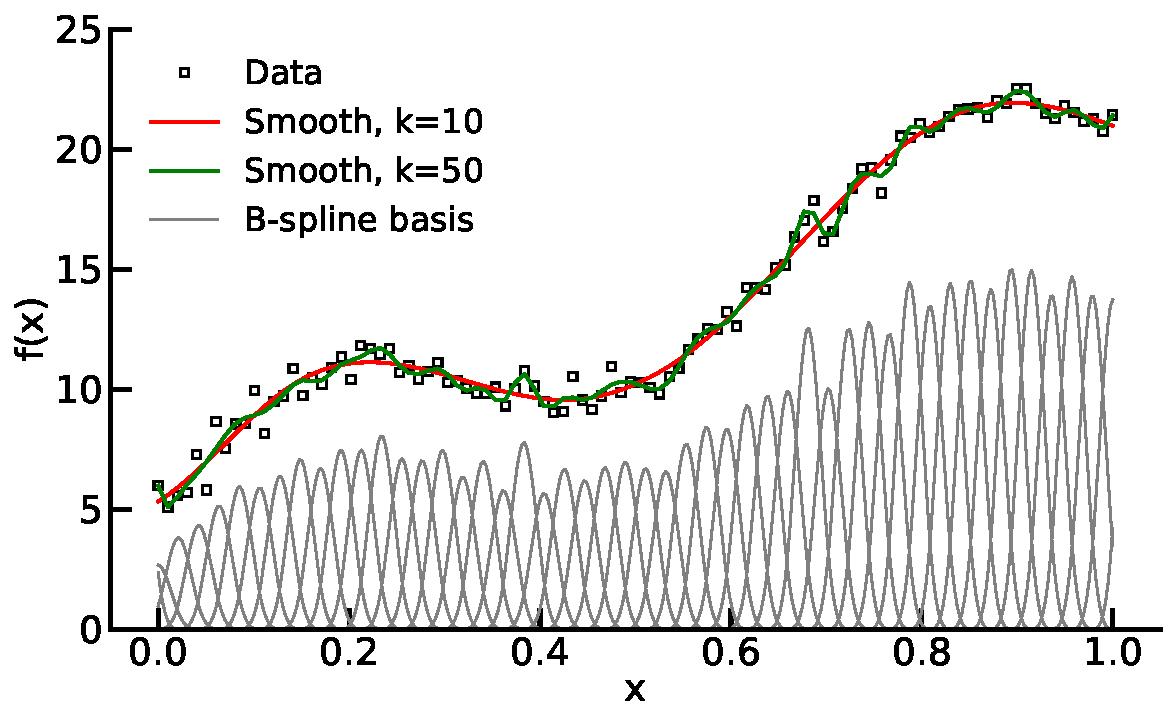
\includegraphics[width=\linewidth]{../thesisplots/smooth_wiggly_bf.pdf}
	\caption{Approximation of the noisy data by 10 and 50 B-splines without constraints}
	\label{fig:smooth_bf_large}
\end{figure}


%%%%%%%%%%%%%%%%%%%%%%%%%%%%%%%%%%%%%%%%%%%%%%%%%%%%%%%%%%%%%%%%%%%%%%%%%%%%%%%%%%%%%%%%%%%%%%%%%%%%%%%%%%%%%%%%%
\subsection{1d Smooth Function Estimation} \label{subsec:1D_smooth}

The second derivative of the estimated function $f(x)$, i.e. $f''(x) = \sum_{j=1}^k B''_i(x) \beta_k$, has to be penalized to realize a smoother estimate when using  a high number of splines. Eilers and Marx have introduced the so-called P-splines. \cite{eilers1996flexible}, see Chapter \ref{subsec:p-splines}. Therefore, the objective function in (\ref{eq:OF_1}) is extended by an additional term considering the smoothness, i.e.

\begin{align}\label{eq:OF_2}
	Q_2(\vec{y}, \vec{\beta}) = Q_1(\vec{y}, \vec{\beta}) + \lambda_s \mathcal{J}_s(\vec{\beta}; d) = \lVert \vec{y} - \vec{X} \vec{\beta} \rVert^2 + \lambda_s \transpose{\vec{\beta}} \transpose{\vec{D}}_d \vec{D}_d \vec{\beta}, 
\end{align}

with the smoothing parameter $\lambda_s$ and an appropriate mapping matrix $\vec{D}_d$ capturing the second derivative, which itself is a measure for function wiggliness. Here, an approximation of the second derivative can be performed by the squared finite difference of order $d$ of adjacent coefficients using the matrix form $\vec{D}_d$ of the difference operator of order $d$, see Chapter \ref{subsec:p-splines}. 

By minimizing the objective function (\ref{eq:OF_2}), i.e.

\begin{align}\label{eq:optimization_problem_2}
	\hat{\vec{\beta}}_{PLS} = \arg \min_{\vec{\beta}} Q_2(\vec{y}, \vec{\beta}),
\end{align}

using the penalized least squares algorithm PLS, the penalized least squares estimates are given by

\begin{align} \label{eq:PLS_coef}
	\hat{\vec{\beta}}_{PLS}= (\transpose{\vec{X}} \vec{X} + \lambda_s \transpose{\vec{D}}_d \vec{D}_d)^{-1} \transpose{\vec{X}} \vec{y}.
\end{align} 
%
In (\ref{eq:PLS_coef}), the smoothing parameter $\lambda_s$ plays a critical role and can be optimized using the information criteria specified in Chapter \ref{subsec:MAC}, e.g. AIC and BIC, or by using cross-validation techniques, see Chapter \ref{subsubsec:Cross-validation}. \cite{fahrmeir2007regression}

For small values $\lambda_s \rightarrow 0$, the penalized least squares estimate $\hat{\vec{\beta}}_{PLS}$ approaches the least squares estimate $\hat{\vec{\beta}}_{LS}$, cf. (\ref{eq:LS_coef}), while for large values $\lambda_s \gg 0$, the fitted function shows the behavior of a polynomial with $d-1$ degrees of freedom. For example, using $d=2$ and a large smoothing parameter $\lambda_s$ this configuration leads to a linear function, while using $d=1$ would lead to a constant function. \cite{fahrmeir2007regression}

Figure \ref{fig:psplines} shows the behavior of P-splines of degree $m=3$ using $k=50$ splines for several values of the smoothing parameter $\lambda_s = \{10^{-2}, 10^{2},10^{5},10^{6}\}$ and a smoothness penalty of order $d=2$.  As the value of $\lambda_s$ gets larger, the fitted curve becomes more smooth and thus the $2^{nd}$ derivative of the curve becomes smaller due to the penalty considered in the estimation, see (\ref{eq:PLS_coef}). For very large values of $\lambda_s$, the estimate approaches a straight line, see the yellow curve in Figure \ref{fig:psplines}.

\begin{figure}[H]
	\centering
	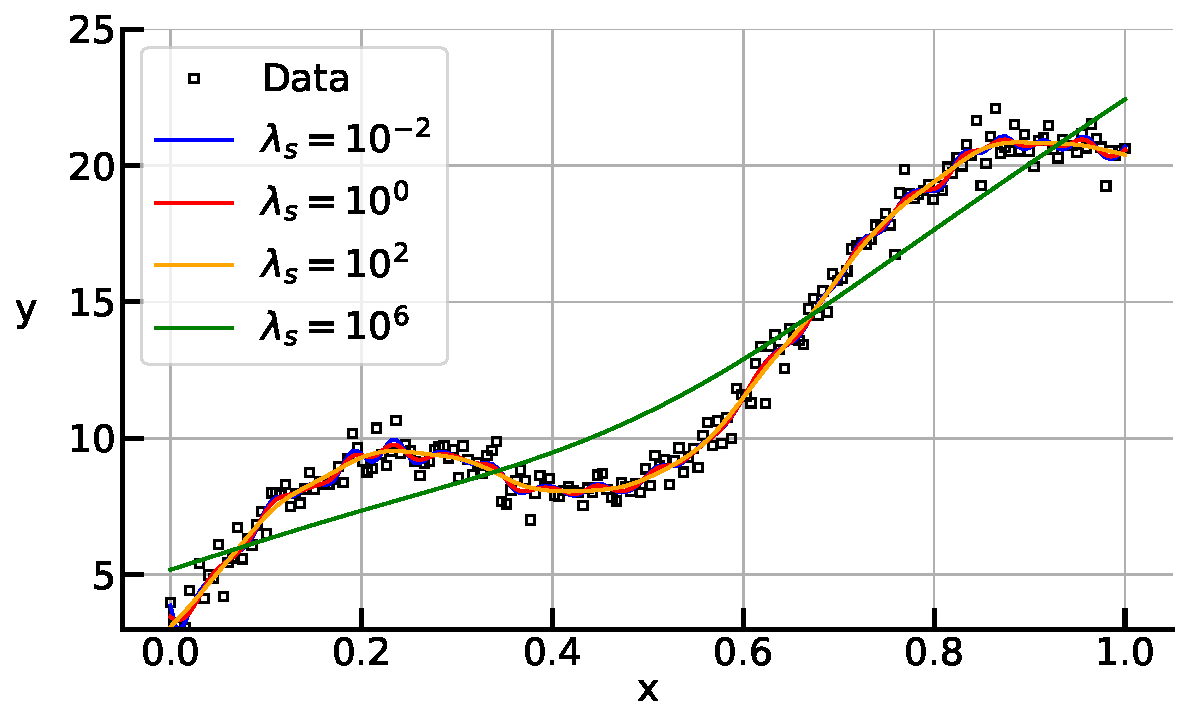
\includegraphics[width=\linewidth]{../thesisplots/p_splines.pdf}
	\caption{Smooth function estimation for different smoothing parameters $\lambda_s$}
	\label{fig:psplines}
\end{figure}

%%%%%%%%%%%%%%%%%%%%%%%%%%%%%%%%%%%%%%%%%%%%%%%%%%%%%%%%%%%%%%%%%%%%%%%%%%%%%%%%%%%%%%%%%%%%%%%%%%%%%%%%%%%%%%%%%
\subsection{1d Constraint Function Estimation}

A priori domain knowledge can now be systematically considered by the extension of the objective function (\ref{eq:OF_2}) using an additional term representing the user-defined constraint, see Table \ref{tab:constraint_overview}. Note that this approach incorporates the a priori knowledge as soft constraints. Therefore, no guarantee can be given that the fit holds the constraint for every possible input. The constraint penalized least-squares objective function is given by

\begin{align}\label{eq:OF_3}
	Q_3(\vec{y}, \vec{\beta}) = Q_1(\vec{y}, \vec{\beta}) + \lambda_s \mathcal{J}_s(\vec{\beta}; d) + \lambda_c \mathcal{J}_c(\vec{\beta}; c)
\end{align}

with the corresponding constraint parameter $\lambda_c$, which determines the influence of the user-defined constraint. Note that the parameter $\lambda_c$ has to be set quite large, i.e. $\lambda_c > 10^4$, compared to $\lambda_s$ to enforce the user-defined constraint. 

Constraints for monotonicity, curvature, unimodality, boundedness and jamming can be modeled as 

\begin{align} \label{eq:mapping_matrix}
	\mathcal{J}_c(\vec{\beta}; c) = \transpose{\vec{\beta}} \transpose{\vec{D}}_c \vec{V} \vec{D}_c  \vec{\beta}
\end{align}

with the mapping matrix $\vec{D}_c$ and the diagonal weighting matrix $\vec{V} := \vec{V}(\vec{\beta}; c)$ capturing if the constraint $c$ is active or inactive. The matrices $\vec{D}_c$ and $\vec{V}$ will further be defined in Chapter \ref{sec:user-defined-constraints}.

By minimizing the objective function (\ref{eq:OF_3}), i.e.

\begin{align}\label{eq:optimization_problem_3}
	\hat{\vec{\beta}}_{PLS, c} = \arg \min_{\vec{\beta}} Q_6(\vec{y}, \vec{\beta}),
\end{align}

the constraint penalized least-squares estimate can be given as

\begin{align} \label{eq:PLS,c_coef}
	\hat{\vec{\beta}}_{PLS, c} = (\transpose{\vec{X}} \vec{X} + \lambda_s \transpose{\vec{D}}_d \vec{D}_d + \lambda_c \transpose{\vec{D}}_c \vec{V} \vec{D}_c)^{-1} \transpose{\vec{X}} \vec{y}.
\end{align}	

Note, (\ref{eq:PLS,c_coef}) is a nonlinear equation because the matrix $\vec{V}$ depends on $\vec{\beta}$. Thus, it has to be solved iteratively to calculate optimal coefficients $\hat{\vec{\beta}}_{PLS,c}$. The algorithm is shown in Figure \ref{fig:pirls}. 

\begin{figure}[H]
	\centering
	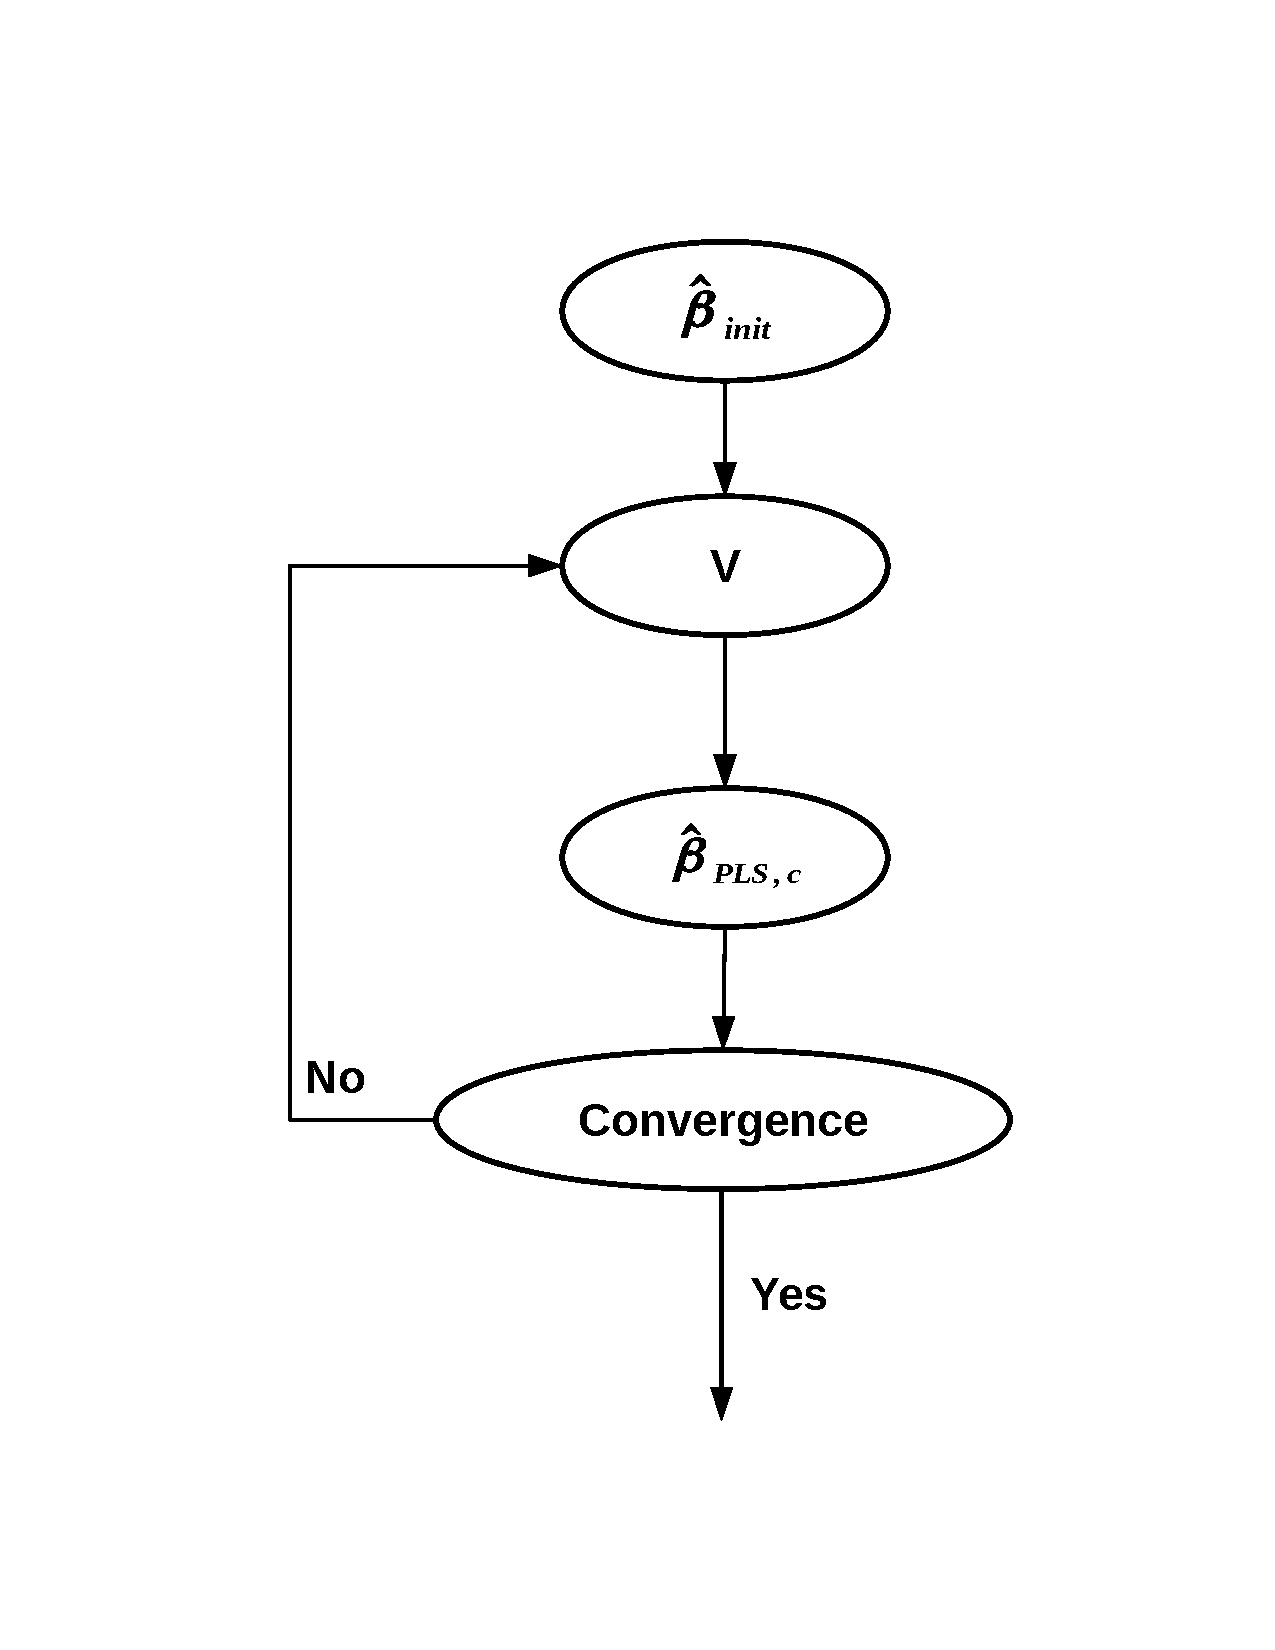
\includegraphics[width=0.6\linewidth]{../thesisplots/algorithm.pdf}
	\caption{Penalized iteratively reweighted least squares algorithm}
	\label{fig:pirls}
\end{figure}


The initial estimate $\hat{\vec{\beta}}_{init}$ needed to compute the weighting matrix $\vec{V}$ is given by the least squares estimate $\hat{\vec{\beta}}_{LS}$. Based on the initial estimate $\hat{\vec{\beta}}_{init}$, the weighting matrix $\vec{V}$ and then the constraint least-squares estimate $\hat{\vec{\beta}}_{PLS,c}$ are calculated. The algorithm is performed until no more changes in the weighting matrix $\vec{V}$ appear. This scheme is called the penalized iteratively reweighted least squares and is abbreviated by PIRLS. \cite{hofner2011monotonicity}


Figure \ref{fig:incspline} shows an example, where the noisy data shown in Figure \ref{fig:test_func} is approximated by considering the monotonicity constraint. The estimate has to be monotonically increasing in contrast to the data, i.e. $f'(x) \ge 0$.  The smoothing parameter $\lambda_s$ was optimized using cross-validation and set to $\lambda_s=271.9$. The constraint parameter $\lambda_c$ was set to $\lambda_c = 6000$. For both function estimations, i.e. using P-splines (blue curve) vs. using constraint P-splines (red curve), the number of used splines $k$ was set to $k=30$. 	

\begin{figure}[H]
	\centering
	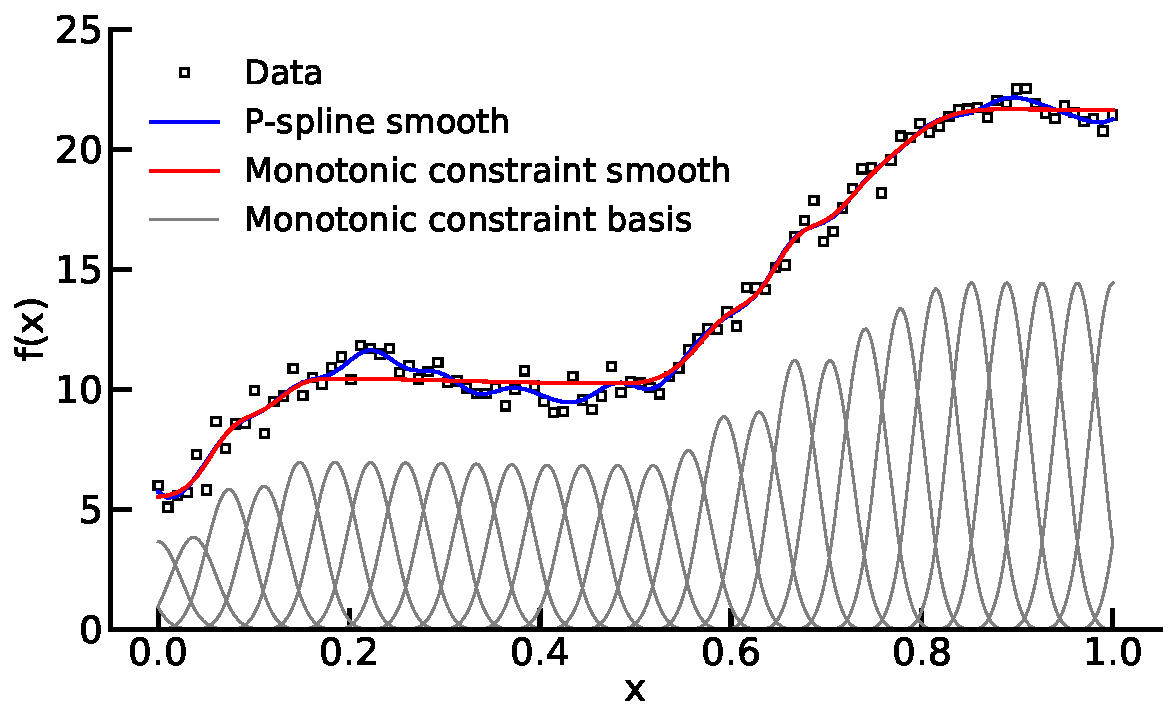
\includegraphics[width=\linewidth]{../thesisplots/inc_spline.pdf}
	\caption{Approximation of the noisy data by P-splines and P-splines with the monotonic increasing constraint}
	\label{fig:incspline}
\end{figure}	

The constraint function estimation (red curve in Figure \ref{fig:incspline}), follows the monotonicity constraint far better that the smooth function estimation (blue curve in Figure \ref{fig:incspline}). For $x < 0.15$ and $x > 0.6$, the two fits are nearly identical, since no constraint violation is present. Note, the entries of the weighting matrix $\vec{V}$ in this region are therefore $0$ because the constraint is not active. For $x \in [0.15, 0.6]$ the constraint is active. The red fit produces an almost constant line in this region as an optimal solution for the competing goals of data accuracy, smoothness and constraint fidelity.

This shows, that the incorporation of a priori knowledge in the fitting process using P-splines is in principle possible using an appropriate choice of the mapping matrix $\vec{D}_c$ and the weighting matrix $\vec{V}$ as well as an iterative fitting approach using penalized iteratively reweighted least squares. These matrices are futher discussed in the following chapters.

%%%%%%%%%%%%%%%%%%%%%%%%%%%%%%%%%%%%%%%%%%%%%%%%%%%%%%%%%%%%%%%%%%%%%%%%%%%%%%%%%%%%%%%%%%%%%%%%%%%%%%%%%%%%%%%%%
%%%%%%%%%%%%%%%%%%%%%%%%%%%%%%%%%%%%%%%%%%%%%%%%%%%%%%%%%%%%%%%%%%%%%%%%%%%%%%%%%%%%%%%%%%%%%%%%%%%%%%%%%%%%%%%%%	
\section{User-defined Constraints} \label{sec:user-defined-constraints}

As stated before, a priori domain knowledge given in Table \ref{tab:constraint_overview} can be introduced by the choice of the mapping matrix $\vec{D}_c$ and the weighting matrix $\vec{V}$, cf. (\ref{eq:mapping_matrix}) and (\ref{eq:PLS,c_coef}). Now a description of the different matrices, which are used to enforce the a priori known domain behavior, is presented. 

%%%%%%%%%%%%%%%%%%%%%%%%%%%%%%%%%%%%%%%%%%%%%%%%%%%%%%%%%%%%%%%%%%%%%%%%%%%%%%%%%%%%%%%%%%%%%%%%%%%%%%%%%%%%%%%%%
\subsection{Monotonicity Constraint}

The mapping matrix $\vec{D}_{monoton}$ enforcing monotonic behavior is given by the first order difference operator $\Delta^1$ for equidistant knot placement, cf. \ref{eq:d1-difference-matrix}. The corresponding matrix for $k$ splines is given as

\begin{align} \label{eq:D_c_monoton}
	\vec{D}_{monoton} = \begin{pmatrix}  -1 & 1  &  		& \\ 
		& -1 & 1 		& \\ 
		&    & \ddots  & \ddots  
	\end{pmatrix} \in \mathbb{R}^{k-1 \times k}.
\end{align}

The difference between monotonic increasing and decreasing behavior is controlled by the weighting matrix $\vec{V}$. For increasing behavior, the weighting matrix $\vec{V}$ is given by the weights $v_j$ according to

\begin{align} \label{eq:v_monoton_inc}
	v_j(\vec{\beta}) = \begin{cases}
			0, \quad \text{if} \ \Delta^1\beta_j \ge 0 \\ 
			1, \quad \text{if} \ \Delta^1\beta_j < 0
	\end{cases}	\ \text{for} \ j=2, \dots, k-1.
\end{align}

For decreasing behavior, the weighting matrix $\vec{V}$ is given by the weights $v_j$ according to
\begin{align} \label{eq:v_monoton_dec}
	v_j(\vec{\beta}) = \begin{cases} 0, \quad \text{if} \ \Delta^1\beta_j \le 0 \\ 
		1, \quad \text{if} \ \Delta^1\beta_j > 0
	\end{cases} \ \text{for} \ j=2, \dots, k-1.
\end{align}

This states, that the penalty term $\mathcal{J}_c(\vec{\beta}; c)$ only contributes if adjacent coefficients $\beta_{j-1}$ and $\beta_j$ are increasing or decreasing, respectively. \cite{hofner2011monotonicity} \cite{eilers2005unimodal}

%%%%%%%%%%%%%%%%%%%%%%%%%%%%%%%%%%%%%%%%%%%%%%%%%%%%%%%%%%%%%%%%%%%%%%%%%%%%%%%%%%%%%%%%%%%%%%%%%%%%%%%%%%%%%%%%%	
\subsection{Curvature Constraint}

In the simplest case, the curvature of the function $f(x)$ can either be convex, i.e. $f''(x) \ge 0$, or concave, i.e. $f''(x) \le 0$. The mapping matrix $\vec{D}_{curvature}$ enforcing this behavior can be approximated by the second order difference operator $\Delta^2$ for equidistant knot placement, cf. (\ref{eq:d2-difference-matrix}). The corresponding matrix for $k$ splines is given as

\begin{align} \label{eq:D_c_curvature}
	\vec{D}_{curvature} = \begin{pmatrix} 1 & -2 & 1 		&  		 & \\ 
		& 1  &-2 	    &1 		 & \\
		& 	  & \ddots  & \ddots & \ddots  
	\end{pmatrix} \in \mathbb{R}^{k-2 \times k}.
\end{align}	

The difference between concave and convex curvature is controlled by the weighting matrix $\vec{V}$. For concave curvature, the weighting matrix $\vec{V}$ is given by the weights $v_j$ according to

\begin{align}\label{eq:v_curvature_concave}
	v_j(\vec{\beta}) = \begin{cases} 
		0, \quad \text{if} \ \Delta^2\beta_j \le 0 \\ 
		1, \quad \text{if} \ \Delta^2\beta_j > 0
	\end{cases} \ \text{for} \ j=1, \dots, k-2.
\end{align}

For convex curvature, the weighting matrix $\vec{V}$ is given by the weights $v_j$ according to

\begin{align}\label{eq:v_curvature_convex}
	v_j(\vec{\beta}) = \begin{cases} 
		0, \quad \text{if} \ \Delta^2\beta_j \ge 0 \\ 
		1, \quad \text{if} \ \Delta^2\beta_j < 0
	\end{cases}\ \text{for} \ j=1, \dots, k-2.
\end{align}	

Therefore, the penalty term $\mathcal{J}_c(\vec{\beta}; c)$ in (\ref{eq:OF_3}) or (\ref{eq:PLS,c_coef}) only contributes if the second order difference of adjacent coefficients $\vec{\beta}$ is either positive or negative, respectively. \cite{eilers2005unimodal}

%%%%%%%%%%%%%%%%%%%%%%%%%%%%%%%%%%%%%%%%%%%%%%%%%%%%%%%%%%%%%%%%%%%%%%%%%%%%%%%%%%%%%%%%%%%%%%%%%%%%%%%%%%%%%%%%%	
\subsection{Unimodality Constraint}

We assume that there is a peak in the data $\{x^{(i)}, y^{(i)}\}$ and therefore want to constrain the fit to include a peak. The peak constraint is given by the unimodal mapping matrix $D_{unimodal}$ and the peak weighting matrix $V$. A function $f(x)$ is said to be unimodal if for some value $m$, it is monotonically increasing for $x \le m$ and monotonically decreasing for $x \ge m$. 

The mapping matrix $\vec{D}_{unimodal}$ enforcing unimodal behavior can be constructed using the first order difference operator $\Delta^1$ for equidistant knot placement, cf. (\ref{eq:d1-difference-matrix}), and is given for $k$ splines as 

\begin{align}\label{eq:D_c_unimodal}
	\vec{D}_{unimodal} = \begin{pmatrix} -1 & 1 \\ 
		& \ddots & \ddots  \\
		& & -1 & 1
	\end{pmatrix} \in \mathbb{R}^{k-1 \times k}
\end{align}

The weighting matrix $\vec{V}$ now has a special structure. First, we construct the B-spline basis using the given data as in Chapter \ref{subsec:b-splines}. We then need to find the index $j_{peak}$ of the \emph{peak spline}, which has the maximal value at the peak data point $\max \{f(x^{(i)}) \ \forall \ i \}$, see Figure \ref{fig:peak_spline}. The index $j_{peak}$ is now used as splitting point for the weighting matrix $\vec{V}$. All coefficients $\beta_j$ for $j < j_{peak}$ are constrained to be monotonic increasing, i.e. $\Delta^1 \beta_j \ge 0$ for $j = 1, \dots, j_{peak}-1$, while all coefficients $\beta_j$ for $j > j_{peak}$ are constrained to be monotonic decreasing, i.e. $\Delta^1 \beta_j \le 0$ for $j = j_{peak}+1, \dots, k$. The coefficient $\beta_{j_{peak}}$ stays unconstrained. \cite{eilers2005unimodal} 

\begin{figure}[H]
	\centering
	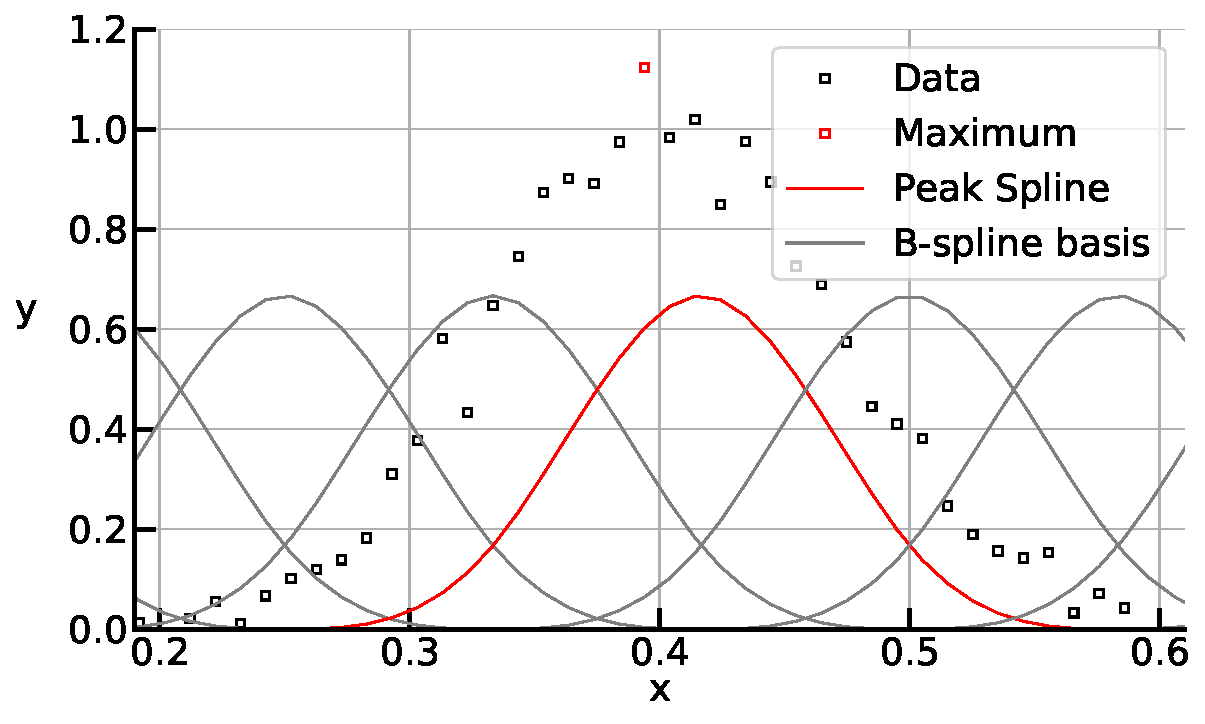
\includegraphics[width=\linewidth]{../thesisplots/peak_spline.pdf}
	\caption{Identification of the peak spline based on data}
	\label{fig:peak_spline}
\end{figure}


The weights $v_j$ to incorporate the peak constraint have the following structure, i.e.

\begin{align}\label{eq:v_peak_1}
	v_j(\vec{\beta}) &= \begin{cases} 
		0, \quad \text{if} \ \Delta^1\beta_j \ge 0 \\ 
		1, \quad \text{if} \ \Delta^1\beta_j  < 0
	\end{cases}, \quad \text{for} \ j=2, \dots, j_{peak}-1
\end{align}

and 

\begin{align}\label{eq:v_peak_2}
	v_j(\vec{\beta}) &= \begin{cases} 
		0, \quad \text{if} \ \Delta^1\beta_j \le 0 \\ 
		1, \quad \text{if} \ \Delta^1\beta_j > 0
	\end{cases}, \quad \text{for} \ j=j_{peak}+1, \dots, k.
\end{align}

The weight $v_{j_{peak}}$ for the \emph{peak spline} is given by $v_{j_{peak}}(\vec{\beta}) = 0$. 

When assuming a valley in the data, the same approach as above can easily be used by multiplying the data with $-1$ or by always doing the inverse operation, i.e. finding the index $j_{valley}$ of the \emph{valley spline}, then constraining all splines for $j < j_{valley}$ to be monotonic decreasing, i.e. $\Delta^1 \beta_j \le 0$ for $j = 1, \dots, j_{valley}-1$, and all splines for $j > j_{valley}$ to be monotonic increasing, i.e. $\Delta^1 \beta_j \ge 0$ for $j = j_{valley}+1, \dots, k$. The coefficient $\beta_{j_{valley}}$ stays unconstrained. 

The weights $v_j$ to consider a valley constraint are given by

\begin{align}\label{eq:v_valley_1}
	v_j(\vec{\beta}) &= \begin{cases} 
		0, \quad \text{if} \ \Delta^1\beta_j \le 0 \\ 
		1, \quad \text{if} \ \Delta^1\beta_j > 0
	\end{cases}, \quad \text{for} \ j=2, \dots, j_{valley}-1
\end{align}

and 

\begin{align}\label{eq:v_valley_2}
	v_j(\vec{\beta}) &= \begin{cases} 
		0, \quad \text{if} \ \Delta^1\beta_j \ge 0 \\ 
		1, \quad \text{if} \ \Delta^1\beta_j < 0.
	\end{cases}, \quad \text{for} \  j=j_{valley}+1, \dots, k.
\end{align}

The weight $v_{j_{valley}}$ for the \emph{valley spline} is given by $v_{j_{valley}}(\vec{\beta}) = 0$.

%%%%%%%%%%%%%%%%%%%%%%%%%%%%%%%%%%%%%%%%%%%%%%%%%%%%%%%%%%%%%%%%%%%%%%%%%%%%%%%%%%%%%%%%%%%%%%%%%%%%%%%%%%%%%%%%
\subsection{Boundedness Constraint}

For certain physical systems, it is known a priori that the measured quantity cannot be smaller than zero, i.e. $f(x) \ge 0$. Using data-driven modeling on noisy data can lead to predictions in the interpolation and extrapolation regime, which may not hold this constraint due to uncertainties captured by the data. It is therefore appropriate to apply the user-defined constraint of boundedness from below.

The user-defined constraint for boundedness from below by $M=0$ uses as mapping matrix $\vec{D}_c$ the B-spline basis matrix $\vec{X} \in \mathbb{R}^{n \times k}$. The weighting matrix $\vec{V} \in \mathbb{R}^{n\times n}$, with individual weights $v_j$, is specified as follows:

\begin{align} \label{eq:v_boundedness}
	v_j(\vec{\beta}) = \begin{cases} 
		0, \quad \text{if} \ f(x^{(j)}) \ge M\\ 
		1, \quad \text{if} \ f(x^{(j)})  < M 		
	\end{cases} \text{for} \ j=1, \dots, n.
\end{align}

Using different values of $M$ allows us to bound from below from any number $M$. Switching the comparison operators in (\ref{eq:v_boundedness}) enables us to bound functions from above. 

%%%%%%%%%%%%%%%%%%%%%%%%%%%%%%%%%%%%%%%%%%%%%%%%%%%%%%%%%%%%%%%%%%%%%%%%%%%%%%%%%%%%%%%%%%%%%%%%%%%%%%%%%%%%%%%%
\subsection{Jamming Constraint}

Jamming the function $f(x)$ by some point $p = \{x^{(jamm)}, y^{(jamm)}\}$ means that the estimated function $f(x^{(jamm)}) \approx y^{(jamm)}$. This can be incorporated using the B-spline basis matrix $\vec{X} \in \mathbb{R}^{n \times k}$ as mapping matrix $\vec{D}_c$ and a weighting matrix $\vec{V} \in \mathbb{R}^{n \times n}$ given by

\begin{align} \label{eq:v_jamming}
	v_j(\vec{\beta}) = 
		\begin{cases}
			0, \quad \text{if} \ x^{(j)} \ne x^{(jamm)} \\
			1, \quad \text{if} \ x^{(j)} = x^{(jamm)} 
	\end{cases} \text{for} \ j = 1, \dots, n.
\end{align} 

%%%%%%%%%%%%%%%%%%%%%%%%%%%%%%%%%%%%%%%%%%%%%%%%%%%%%%%%%%%%%%%%%%%%%%%%%%%%%%%%%%%%%%%%%%%%%%%%%%%%%%%%%%%%%%%%
\subsection{Penalty Term for Tensor-Product Splines}

To extend the framework of mapping matrices to two dimensions and tensor-product splines, we again use the concept of Kronecker products given in Chapter \ref{subsubsec:tp-splines}. In principle, every possible pair of one dimensional user-defined constraints can be constructed using the approach in Chapter \ref{subsubsec:tp-splines}, e.g. unimodality in two dimensions would be obtained using the unimodal mapping matrix depicted above for each dimension. We then also need to include the constraint specific weight matrices $\vec{V}$.

The penalty term for the constraint given by $c_1$ for dimension $1$ and $c_2$ for dimension $2$ then has the form

\begin{align} \label{eq:J-c-tps}
	\mathcal{J}_c(\vec{\beta}; c) = \transpose{\vec{\beta}} \Big[ \vec{I}^2 \otimes \vec{K}_{c_1} + \vec{K}_{c_2} \otimes \vec{I}^1\Big] \vec{\beta}
\end{align}

with the respective penalty matrices $\vec{K}_{c_1} = \vec{D}_{c_1}^{\text{T}} \vec{V}_1 \vec{D}_{c_1}$ for dimension $x_1$ and $\vec{K}_{c_2} = \vec{D}_{c_2}^{\text{T}} \vec{V}_2 \vec{D}_{c_2}$ for dimension $x_2$ using the weighting matrices $\vec{V}_1$ and $\vec{V}_2$, the mapping matrices $\vec{D}_{c_1}$ and $\vec{D}_{c_2}$ and the identity matrices $\vec{I}^1$ and $\vec{I}^2$ for the respective dimension.

%%%%%%%%%%%%%%%%%%%%%%%%%%%%%%%%%%%%%%%%%%%%%%%%%%%%%%%%%%%%%%%%%%%%%%%%%%%%%%%%%%%%%%%%%%%%%%%%%%%%%%%%%%%%%%%%%
%%%%%%%%%%%%%%%%%%%%%%%%%%%%%%%%%%%%%%%%%%%%%%%%%%%%%%%%%%%%%%%%%%%%%%%%%%%%%%%%%%%%%%%%%%%%%%%%%%%%%%%%%%%%%%%%%
\section{n-d Constraint Function Estimation}

The extension from one input to multiple input dimensions uses the concept of additive models given in Chapter \ref{subsubsec:STAR}. Given input data $\{ x_1^{(i)}, \dots, x_q^{(i)}; y^{(i)}\}, \ i = 1, \dots, n$ and $q$ as the number of inputs, the combined model using all available B-splines and tensor-product splines is given, cf. (\ref{eq:STAR}), as

\begin{align} \label{eq:tps_all}
	y = f(x_1,..., x_q) = \sum_{j=1}^q s_j(x_j) + \sum_{j=1}^{q-1} \sum_{r>j}^q t_{j, r}(x_j, x_r)
\end{align}

where $s_j(x_j)$ is the B-spline estimate given by $s_j(x_j) = \vec{X}_{s_j} \vec{\beta}_{s_j}$ and $t_{j, r}(x_j,x_r)$ is the tensor-product estimate is given by $t_{j, r}(x_j,x_r) = \vec{X}_{t_{j,r}} \vec{\beta}_{t_{j, r}}$. The number of individual estimates is given by 

\begin{align}
	n_{total} = q + \frac{q(q-1)}{2}.  
\end{align}

The constrained penalized least squares objective function for additive models can now be written similar to (\ref{eq:OF_3}) as

\begin{align}\label{eq:OF_6}
	Q_6(\vec{y}, \vec{\beta}) = Q_1(\vec{y}, \vec{\beta}) + \transpose{\vec{\lambda}}_s	\vec{\mathcal{J}}_s(\vec{\beta}; \vec{d}) + \transpose{\vec{\lambda}}_c \vec{\mathcal{J}}_c(\vec{\beta}; \vec{c}).
\end{align}

with $\vec{\lambda}_s \in \mathbb{R}^{n_{total}}$ and  $\vec{\lambda}_c \in \mathbb{R}^{n_{total}}$  defined as vectors with one value of smoothness and constraint parameter for each individual estimate, respectively. 

We now need to specify the three parts of the objective function in (\ref{eq:OF_6}). 

%%%%%%%%%%%%%%%%%%%%%%%%%%%%%%%%%%%%%%%%%%%%%%%%%%%%%%%%%%%%%%%%%%%%%%%%%%%%%%%%%%%%%%%%%%%%%%%%%%%%%%%%%%%%%%%%%
\subsection{Data Term}

Assuming the use of $k$ splines for the B-spline estimates and $k^2$ splines for the tensor-product estimates, the total number of coefficients to be determined is given by 

\begin{align}\label{eq:tps_total_number_of_coef}
	k_{total} = qk + \frac{q(q-1)}{2}k^2. 
\end{align}

Since all B-spline and tensor-product spline models follow a linear model structure, see Chapter \ref{subsec:b-splines} and \ref{subsubsec:tp-splines}, we can combine them into one large model, cf. (\ref{eq:STAR-block-diag}), given by

\begin{align}\label{eq:tps_lin_mod}
	\vec{y} = \vec{X} \vec{\beta}
\end{align}

where the matrix $\vec{X} \in \mathbb{R}^{n \times k_{total}}$ is given in (\ref{eq:STAR-block-diag}) as horizontal concatenation of the individual bases and the combined coefficient vector $\vec{\beta} \in \mathbb{R}^{k_{total}}$ is given in (\ref{eq:STAR-block-diag}) by a vertical concatenation of the individual coefficient vectors. 

The data term $Q_1(\vec{y}, \vec{\beta})$ in the constrained penalized least squares objective function given in (\ref{eq:OF_6}) can now be evaluated using arbitrary input dimensions. 

%%%%%%%%%%%%%%%%%%%%%%%%%%%%%%%%%%%%%%%%%%%%%%%%%%%%%%%%%%%%%%%%%%%%%%%%%%%%%%%%%%%%%%%%%%%%%%%%%%%%%%%%%%%%%%%%%
\subsection{Smoothness Term}

The combined smoothness penalty term $\vec{\mathcal{J}}_s(\vec{\beta}; \vec{d}) \in \mathbb{R}^{n_{total}}$ is then given as

\begin{align}\label{eq:J_s_ndim}
	\vec{\mathcal{J}}_s(\vec{\beta}; \vec{d}) &= 
	\begin{pmatrix}
		\mathcal J_{s_1}(\vec{\beta}_{s_1}; d_{s_1}) \\ 
		\vdots \\ 
		\mathcal J_{s_q}(\vec{\beta}_{s_q}; d_{s_q}) \\
		\mathcal J_{t_{1,2}}(\vec{\beta}_{t_{1,2}}; d_{t_{1,2}}) \\
		\vdots \\
		\mathcal J_{t_{q-1,q}}(\vec{\beta}_{t_{q-1,q}}; d_{t_{q-1,q}}) \\
	\end{pmatrix}
\end{align}

with $\mathcal J_e(\vec{\beta}_e; d_e) = \transpose{\vec{\beta}}_e \transpose{\vec{D}}_{d_e} \vec{D}_{d_e} \vec{\beta}_e$ determining the smoothness penalty term using the coefficients $\vec{\beta}_e$ and mapping matrix $\vec{D}_{d_e}$, see Chapter \ref{subsec:p-splines} and Chapter \ref{subsubsec:tp-splines}, for each estimate $e \in \{s_1, \dots, s_q, t_{1,2}, \dots, t_{q-1,q}\}$. The vector $\vec{d} \in \mathbb{R}^{n_{total}}$ consists of the orders $d_e$ determining the mapping matrix $\vec{D}_{d_e}$ of the smoothness constraint for each individual estimate $e$. 

%%%%%%%%%%%%%%%%%%%%%%%%%%%%%%%%%%%%%%%%%%%%%%%%%%%%%%%%%%%%%%%%%%%%%%%%%%%%%%%%%%%%%%%%%%%%%%%%%%%%%%%%%%%%%%%%%
\subsection{Constraint Term}
The combined constraint penalty term $\vec{\mathcal{J}}_c(\vec{\beta}; \vec{c}) \in \mathbb{R}^{n_{total}}$ is then given as

\begin{align}\label{eq:J_c_ndim}
	\vec{\mathcal{J}}_c(\vec{\beta}; \vec{c}) &= 
	\begin{pmatrix}
		\mathcal J_{s_1}(\vec{\beta}_{s_1}; c_{s_1}) \\ 
		\vdots \\ 
		\mathcal J_{s_q}(\vec{\beta}_{s_q}; c_{s_q}) \\
		\mathcal J_{t_{1,2}}(\vec{\beta}_{t_{1,2}}; c_{t_{1,2}}) \\
		\vdots \\
		\mathcal J_{t_{q-1,q}}(\vec{\beta}_{t_{q-1,q}}; c_{t_{q-1,q}}) \\
	\end{pmatrix}
\end{align}

with $\mathcal J_e(\vec{\beta}_e; c_e) = \transpose{\vec{\beta}}_e \transpose{\vec{D}}_{c_e} \vec{V}_{c_e} \vec{D}_{c_e} \vec{\beta}_e$ determining the constraint penalty term using the coefficients $\vec{\beta}_e$, the mapping matrix $\vec{D}_{c_e}$ and the weighting matrix $\vec{V}_e$ for each estimate $e \in \{s_1, \dots, s_q, t_{1,2}, \dots, t_{q-1,q}\}$, see Chapter (\ref{sec:user-defined-constraints}). The vector $\vec{c} \in \mathbb{R}^{n_{total}}$ consists of the constraint type $c_e$, e.g. monoton increasing, determining the mapping matrix $\vec{D}_{c_e}$ for each individual estimate $e$. 

%%%%%%%%%%%%%%%%%%%%%%%%%%%%%%%%%%%%%%%%%%%%%%%%%%%%%%%%%%%%%%%%%%%%%%%%%%%%%%%%%%%%%%%%%%%%%%%%%%%%%%%%%%%%%%%%%

The objective function (\ref{eq:OF_6}) is then optimized, i.e.

\begin{align}\label{eq:optimization_problem_6}
	\hat{\vec{\beta}}_{PLS,c,nd} = \arg \min_{\vec{\beta}} Q_6(\vec{y}, \vec{\beta}),
\end{align}

using the penalized iteratively reweighted least squares algorithm, cf. (\ref{eq:PLS,c_coef}), to obtain the coefficients $\hat{\vec{\beta}}_{PLS,c,nd}$ as

\begin{align} \label{eq:beta-pls-c-nd-formula}
	\hat{\vec{\beta}}_{PLS,c,nd} = (\transpose{\vec{X}} \vec{X} +\vec{K}_s + \vec{K}_c)^{-1} \transpose{\vec{X}} \vec{y}. 
\end{align}

In (\ref{eq:beta-pls-c-nd-formula}), $\vec{X} \in \mathbb{R}^{n \times k_{total}}$ is the combined basis matrix, cf. (\ref{eq:STAR-block-diag}), $\vec{K}_s \in \mathbb{R}^{k_{total} \times k_{total}}$ is the combined smoothness matrix given as

\begin{align} \label{eq:combined-smoothness-matrix}
	\vec{K}_s = \rotatebox{-90}{$\begin{pmatrix} 
					\lambda_{s_1} \transpose{\vec{D}_{d_{s_1}}} \vec{D}_{d_{s_1}} & 0 \\
					 							0 						  &	\ddots & 0 \\
					 													  &  0 	   & \lambda_{s_q} \transpose{\vec{D}_{d_{s_q}}} \vec{D}_{d_{s_q}} & 0 \\
					 													  &        &           0										   & \lambda_{s_{1,2}} \transpose{\vec{D}_{d_{t_{1,2}}}} \vec{D}_{d_{t_{1,2}}} & 0 \\
					 													  &  & &    0 & \ddots & 0 \\
					 													  &  & &      &   0    & \lambda_{s_{q-1,q}} \transpose{\vec{D}_{d_{t_{q-1,q}}}} \vec{D}_{d_{t_{q-1,q}}}
			\end{pmatrix}$} 
\end{align}

and $\vec{K}_c \in \mathbb{R}^{k_{total} \times k_{total}}$ is the combined constraint matrix as 

\begin{align} \label{eq:combined-constraint-matrix}
	\vec{K}_c = \rotatebox{-90}{$\begin{pmatrix} 
					\lambda_{c_1} \transpose{\vec{D}_{c_{s_1}}} \vec{V}_{c_{s_1}} \vec{D}_{c_{s_1}} & 0 \\
													 			0 						& \ddots & 0 \\
													 			                 		&  0 	 & \lambda_{c_q} \transpose{\vec{D}_{c_{s_q}}} \vec{V}_{c_{s_q}} \vec{D}_{c_{s_q}} & 0 \\
													 			                 		&        &           0										    & \lambda_{c_{1,2}} \transpose{\vec{D}_{c_{t_{1,2}}}} \vec{V}_{c_{t_{1,2}}} \vec{D}_{c_{t_{1,2}}} & 0 \\
													 			                 		& &  &   0 & \ddots & 0 \\
																			         	& &  & 	   &	0   & \lambda_{c_{q-1,q}} \transpose{\vec{D}_{c_{t_{q-1,q}}}} \vec{V}_{c_{t_{q-1,q}}} \vec{D}_{c_{t_{q-1,q}}}
	\end{pmatrix}$}. 
\end{align}




%%%%%%%%%%%%%%%%%%%%%%%%%%%%%%%%%%%%%%%%%%%%%%%%%%%%%%%%%%%%%%%%%%%%%%%%%%%%%%%%%%%%%%%%%%%%%%%%%%%%%%%%%%%%%%%%%%%
\subsection{2-d Example} \label{subsec:2d-example}

As example for the n-d constraint function estimation, we take a look at the function 

\begin{align} \label{eq:2d_test_func}
	f(x_1, x_2) = 2\exp{\Big(-\frac{(x_1 - 0.25)^2}{0.08}\Big)} + x_2^2 + \eta
\end{align}

for $x_1 \in [0,1]$ and $x_2 \in [0,1]$ and random Gaussian noise $\eta$ with $\sigma_{noise} = 0.1$. Therefore we expect a peak in dimension $x_1$ as well as increasing behavior for dimension $x_2$, see Figure \ref{fig:2d_example}. The user-defined constraints are therefore $c_1 = \text{unimodal}$ and $c_2 = \text{monotonic increasing}$ Using this knowledge, we create a model with the following characteristics:

\begin{itemize}
	\item B-spline smooth $s_1(x_1)$: $k_{x_1} = 50$, $c = c_1$, $\lambda_s = 1$ and $\lambda_c = 6000$
	\item B-spline smooth $s_2(x_2)$: $k_{x_2} = 50$, $c = c_2$, $\lambda_s = 1$ and $\lambda_c = 6000$
\end{itemize}

The fit for this model as well as the individual estimates $s_1(x_1)$ and $s_2(x_2)$ are shown in Figure \ref{fig:2d_example}. The model fits the data quite well and holds the specified constraints for the individual dimensions.

\begin{figure}[H]
	\centering
	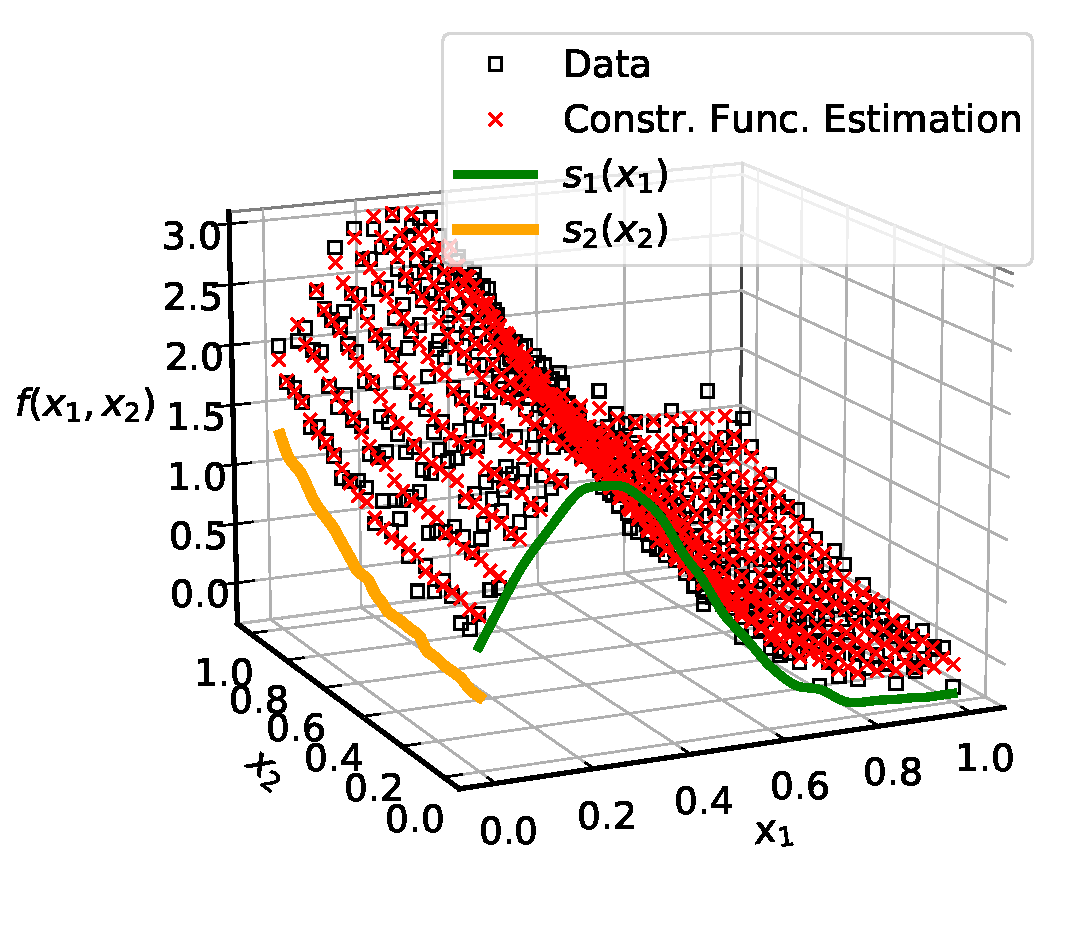
\includegraphics[width=\linewidth]{../thesisplots/2d_example.pdf}
	\caption{2-d test function for n-d constrained function estimation}
	\label{fig:2d_example}
\end{figure}

%%%%%%%%%%%%%%%%%%%%%%%%%%%%%%%%%%%%%%%%%%%%%%%%%%%%%%%%%%%%%%%%%%%%%%%%%%%%%%%%%%%%%%%%%%%%%%%%%%%%%%%%%%%%%%%%%%%%%%%%%%%%%%%%%%%%%%%%%%%%%%%%%%%%%%%%%%%%%%%%%%%%%%%%%%%%%%%%%%%%%%%%%%%%%%%%%%%%%%%%%%%%%%%%%%%%%%%%%%%%%%%%%%%%%%

%\bibliographystyle{IEEEtranN}
%\bibliography{bibliography}

\printbibliography


\end{document}